\documentclass[UTF8,zihao=-4]{ctexart}

\usepackage[a4paper,margin=2.35cm]{geometry}
\usepackage{amsmath,amssymb}
\usepackage{booktabs}
\usepackage{array}
\usepackage{graphicx}
\usepackage{subcaption}
\usepackage{float}
\usepackage{caption}
\usepackage{xcolor}
\usepackage{hyperref}
\usepackage{enumitem}
\usepackage{multirow}

\hypersetup{
  colorlinks=true,
  linkcolor=blue!55!black,
  citecolor=blue!55!black,
  urlcolor=blue!55!black
}

\captionsetup{font=small,labelfont=bf}
\setlist[itemize]{leftmargin=2em,itemsep=0.18em}
\setlist[enumerate]{leftmargin=2em,itemsep=0.18em}
\renewcommand{\arraystretch}{1.16}
\graphicspath{{project_report_figures/}}

\title{\bfseries 双边平台竞争中的网络效应与市场锁定\\项目实验报告}
\author{USTC\_MM26 Final Project}
\date{\today}

\begin{document}
\maketitle

\begin{abstract}
本项目围绕“双边平台竞争中的网络效应与市场锁定”问题，分三个阶段构建并完善实验体系，系统研究用户侧与商户侧交叉网络效应下的平台份额演化、市场锁定机制、策略干预效果以及个体异质性影响。第一阶段基于 Logit 选择与动态调整模型，建立双边平台竞争的基础 ODE 框架，刻画平台 A 的用户份额与商户份额随时间演化的过程。通过基础动态演化、网络效应强度、初始规模差异、服务质量差异和补贴策略实验，验证了双边网络效应能够放大早期优势，并在强网络效应下形成明显路径依赖和市场锁定。实验表明，单侧网络效应不足以稳定地产生赢家通吃，真正的锁定主要来自用户侧和商户侧的相互强化；弱势平台若希望逆转竞争格局，需要在服务质量或补贴强度上跨过一定临界阈值。

第二阶段在基础模型上进一步开展提高型实验，重点识别市场结构变化和策略干预的临界条件。通过市场锁定区域扫描、弱势平台逆袭阈值、双边补贴分配、阶段性补贴退出和利润约束实验，项目从“机制验证”推进到“策略评估”。实验发现，双边网络效应存在清晰的分区边界：当网络效应较弱时平台可以共存，网络效应增强后市场先进入倾斜区，再进一步进入锁定区。弱势平台的逆袭难度会随网络效应和切换成本上升而增加；补贴策略的关键不在于单纯提高补贴总量，而在于能否帮助平台跨越临界规模。阶段性补贴实验说明，补贴可以作为早期跨越门槛的工具，而不必长期持续；利润约束实验进一步表明，过高补贴虽然能维持市场份额，却会因成本过大降低整体收益，因此最优策略往往是“刚好足以跨过临界规模”的中等补贴。

第三阶段引入 Mesa 多智能体 ABM 模型，从微观主体层面对前两阶段的平均场结论进行扩展和机制解释。ABM 将用户和商户建模为具有异质偏好、惯性、补贴敏感度和随机扰动的 agent，并进一步加入精准补贴、冷启动资源配置和商户多归属机制。实验结果表明，个体异质性会改变市场锁定概率和集中程度；在等预算条件下，双边精准补贴比统一补贴和随机补贴更有效；冷启动成功依赖用户侧与商户侧资源共同达到启动边界；低成本多归属能够削弱平台锁定并提高平台共存概率。ABM 实验补充说明，平台竞争结果并非只由平均网络效应决定，还受到个体差异、补贴投向、种子质量和商户经营方式的共同影响。

总体来看，本项目形成了从基础动态建模、临界阈值识别到多智能体机制分析的完整实验链条。实验共同揭示：双边平台竞争具有显著的非线性、路径依赖和临界跃迁特征；平台策略应围绕双边网络效应的启动门槛展开，而不是单纯追求短期份额最大化。研究结果可为平台补贴设计、冷启动资源配置、商户多平台经营以及用户平台选择提供解释依据和策略参考。
\end{abstract}

\noindent\textbf{关键词：} 双边平台；交叉网络效应；市场锁定；临界阈值；补贴策略；Agent-Based Model

\section{研究背景与实验目标}

双边平台同时连接用户侧与商户侧，典型例子包括外卖平台、电商平台、网约车平台和本地生活平台。平台竞争并不是单边需求竞争，而是由两类主体之间的交叉网络效应共同决定：商户越多，用户越愿意进入平台；用户越多，商户越愿意入驻平台。这类机制是双边市场理论的核心问题之一 \cite{rochet2003,armstrong2006,parker2005}。同时，网络外部性和递增收益会带来路径依赖与锁定现象 \cite{katz1985,arthur1989}，使早期微小优势被持续放大。

根据项目实验设计文档《双边平台竞争中的网络效应与市场锁定：分阶段实验设置与实现方式》，本项目不以真实平台数据拟合和精确预测为目标，而是从机制出发建立模型。参数取值依据现实背景、文献机制和合理假设设定，用于覆盖弱、中、强网络效应，以及不同补贴、切换成本和冷启动条件。实验重点是通过多组参数扫描、敏感性分析和多智能体仿真，解释平台共存、市场倾斜、赢家通吃和弱势平台逆袭的形成条件。

项目分为三个阶段：
\begin{enumerate}
  \item 第一阶段：构建基础 ODE 动态模型，验证网络效应、初始优势、服务质量和补贴对市场演化的影响。
  \item 第二阶段：开展提高型实验，识别临界阈值、补贴分配、补贴退出和利润约束下的策略边界。
  \item 第三阶段：引入 Mesa ABM 多智能体仿真，刻画个体异质性、精准补贴、冷启动和商户多归属机制。
\end{enumerate}

\section{统一基础模型}

\subsection{状态变量与效用函数}

设平台 A 的用户份额为 $u(t)$，商户份额为 $m(t)$，平台 B 的对应份额分别为 $1-u(t)$ 和 $1-m(t)$。用户选择平台 A 和 B 的效用分别为
\begin{equation}
V_A^U=q_A^U+\alpha m+b_A^U-p_A^U+s_Uu,
\end{equation}
\begin{equation}
V_B^U=q_B^U+\alpha(1-m)+b_B^U-p_B^U+s_U(1-u).
\end{equation}
商户选择平台 A 和 B 的效用分别为
\begin{equation}
V_A^M=q_A^M+\beta u+b_A^M-r_A+s_Mm,
\end{equation}
\begin{equation}
V_B^M=q_B^M+\beta(1-u)+b_B^M-r_B+s_M(1-m).
\end{equation}
其中，$\alpha$ 表示商户规模对用户吸引力的影响，$\beta$ 表示用户规模对商户吸引力的影响；$q$ 表示服务质量，$b$ 表示补贴，$p$ 和 $r$ 分别表示用户侧价格和商户侧抽成，$s_U,s_M$ 表示切换成本或锁定效应。

\subsection{Logit 选择与动态调整}

用户和商户按照 Logit 规则选择平台 A：
\begin{equation}
P_A^U=\frac{e^{\gamma_U V_A^U}}{e^{\gamma_U V_A^U}+e^{\gamma_U V_B^U}},\qquad
P_A^M=\frac{e^{\gamma_M V_A^M}}{e^{\gamma_M V_A^M}+e^{\gamma_M V_B^M}}.
\end{equation}
市场份额按照当前选择概率与已有份额之间的差距调整：
\begin{equation}
\frac{du}{dt}=\lambda_U(P_A^U-u),\qquad
\frac{dm}{dt}=\lambda_M(P_A^M-m).
\end{equation}
综合份额定义为
\begin{equation}
L_A(t)=\frac{u(t)+m(t)}{2}.
\end{equation}
市场集中度定义为
\begin{equation}
C=|u_A(\infty)-0.5|+|m_A(\infty)-0.5|.
\end{equation}
当 $C<0.2$ 时判定为平台共存，$0.2\le C<0.8$ 判定为市场倾斜，$C\ge 0.8$ 判定为市场锁定。

\section{第一阶段：基础机制实验}

\subsection{实验设计}

第一阶段围绕五个基础问题展开：平台份额如何动态演化；双边网络效应是否导致锁定；初始规模优势是否会被放大；服务质量差异能否帮助弱势平台逆袭；补贴是否存在突破阈值。该阶段采用 ODE 平均场模型，主要目标是验证模型机制是否符合双边平台竞争的基本逻辑。

\begin{figure}[H]
  \centering
  \begin{subfigure}{0.49\textwidth}
    \centering
    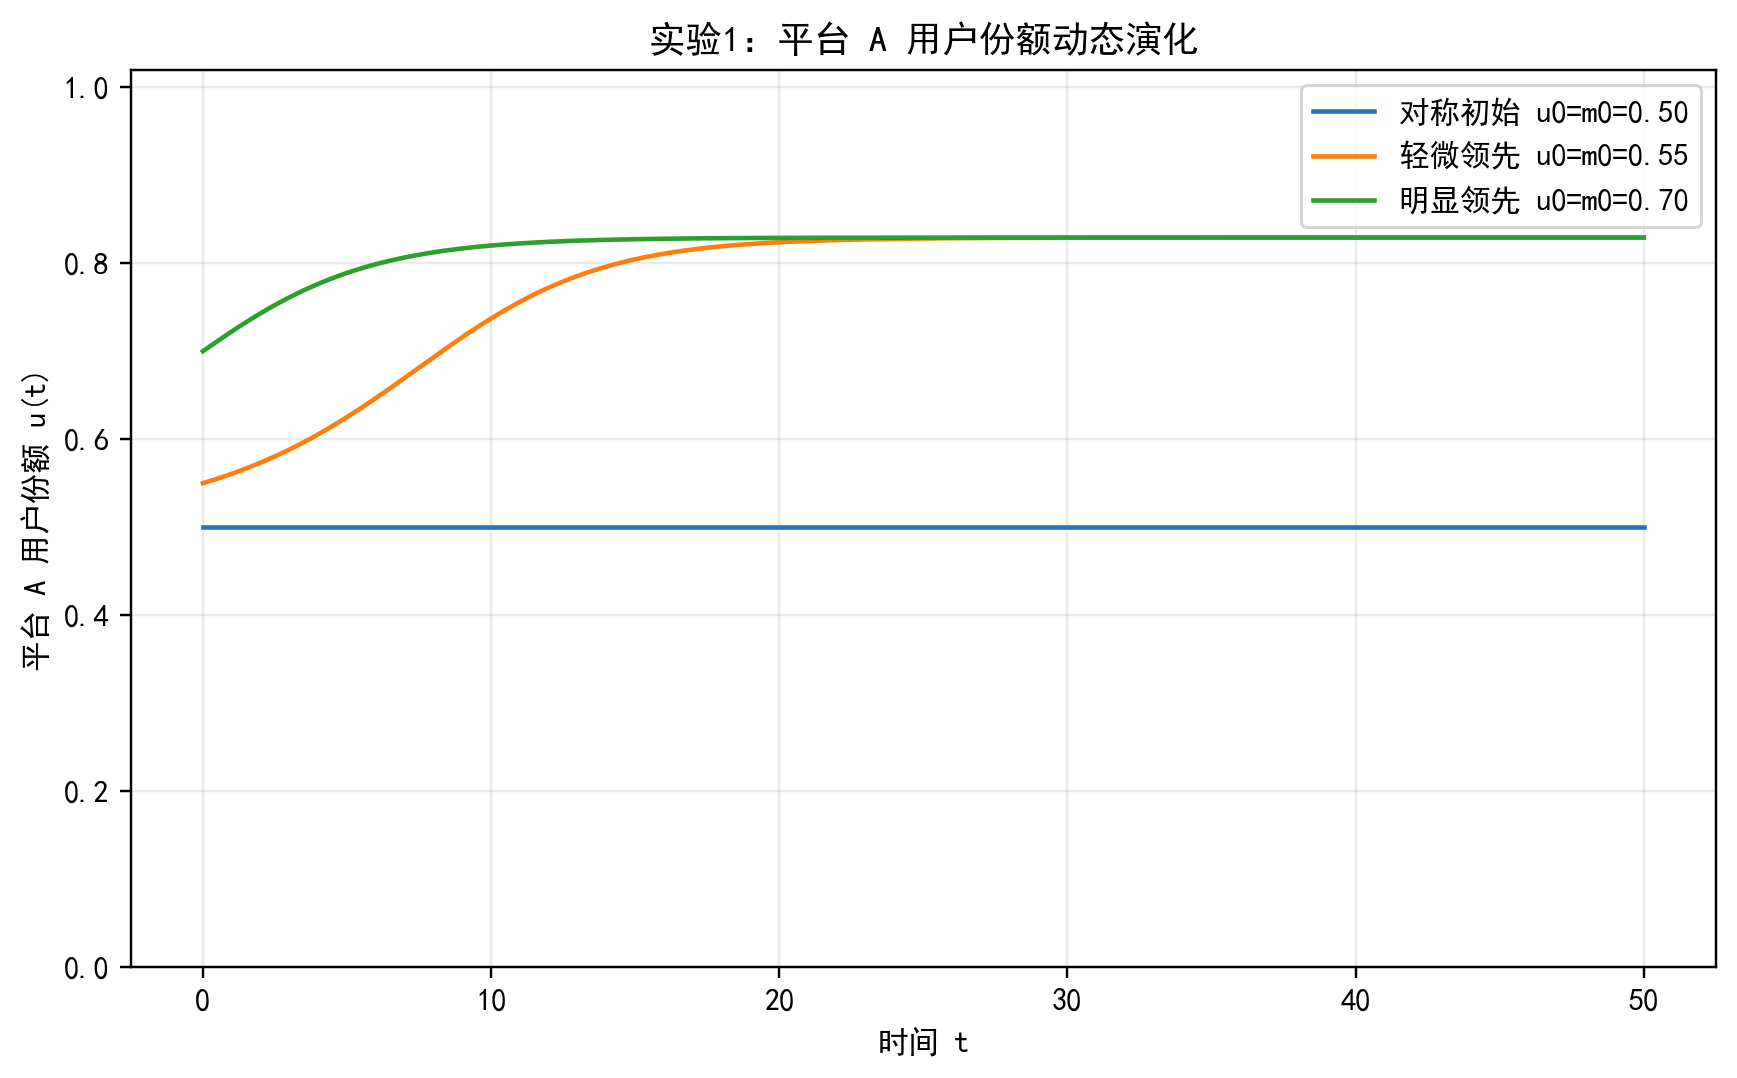
\includegraphics[width=\textwidth]{stage1_exp1_user.png}
    \caption{用户份额动态}
  \end{subfigure}
  \hfill
  \begin{subfigure}{0.49\textwidth}
    \centering
    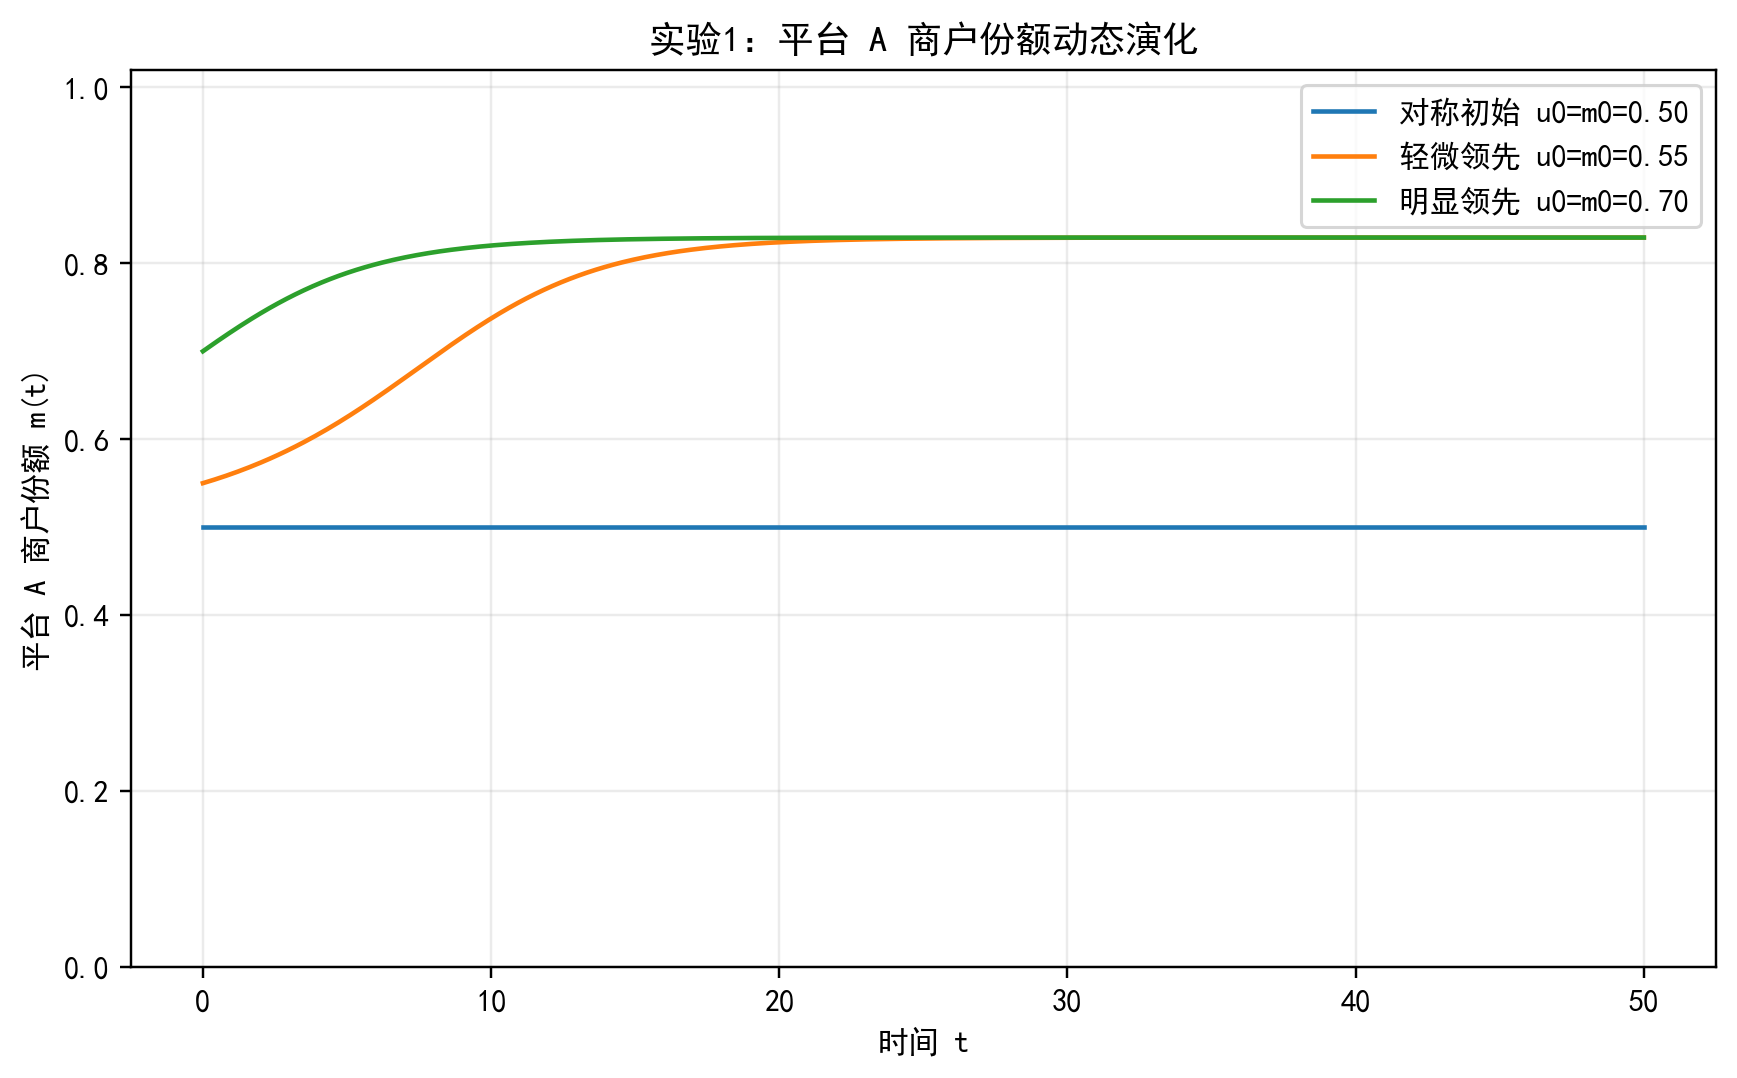
\includegraphics[width=\textwidth]{stage1_exp1_merchant.png}
    \caption{商户份额动态}
  \end{subfigure}
  \caption{阶段一实验 1：基础动态演化}
  \label{fig:stage1-dynamics}
\end{figure}

图 \ref{fig:stage1-dynamics} 表明，在完全对称初始条件下，系统可以维持共存；当平台 A 具有轻微初始优势时，双边网络效应会进一步放大该优势，使用户侧和商户侧份额同步上升。这说明模型能够刻画双边平台中“需求吸引供给、供给反过来吸引需求”的反馈链条。

\subsection{网络效应、初始优势与路径依赖}

\begin{figure}[H]
  \centering
  \begin{subfigure}{0.49\textwidth}
    \centering
    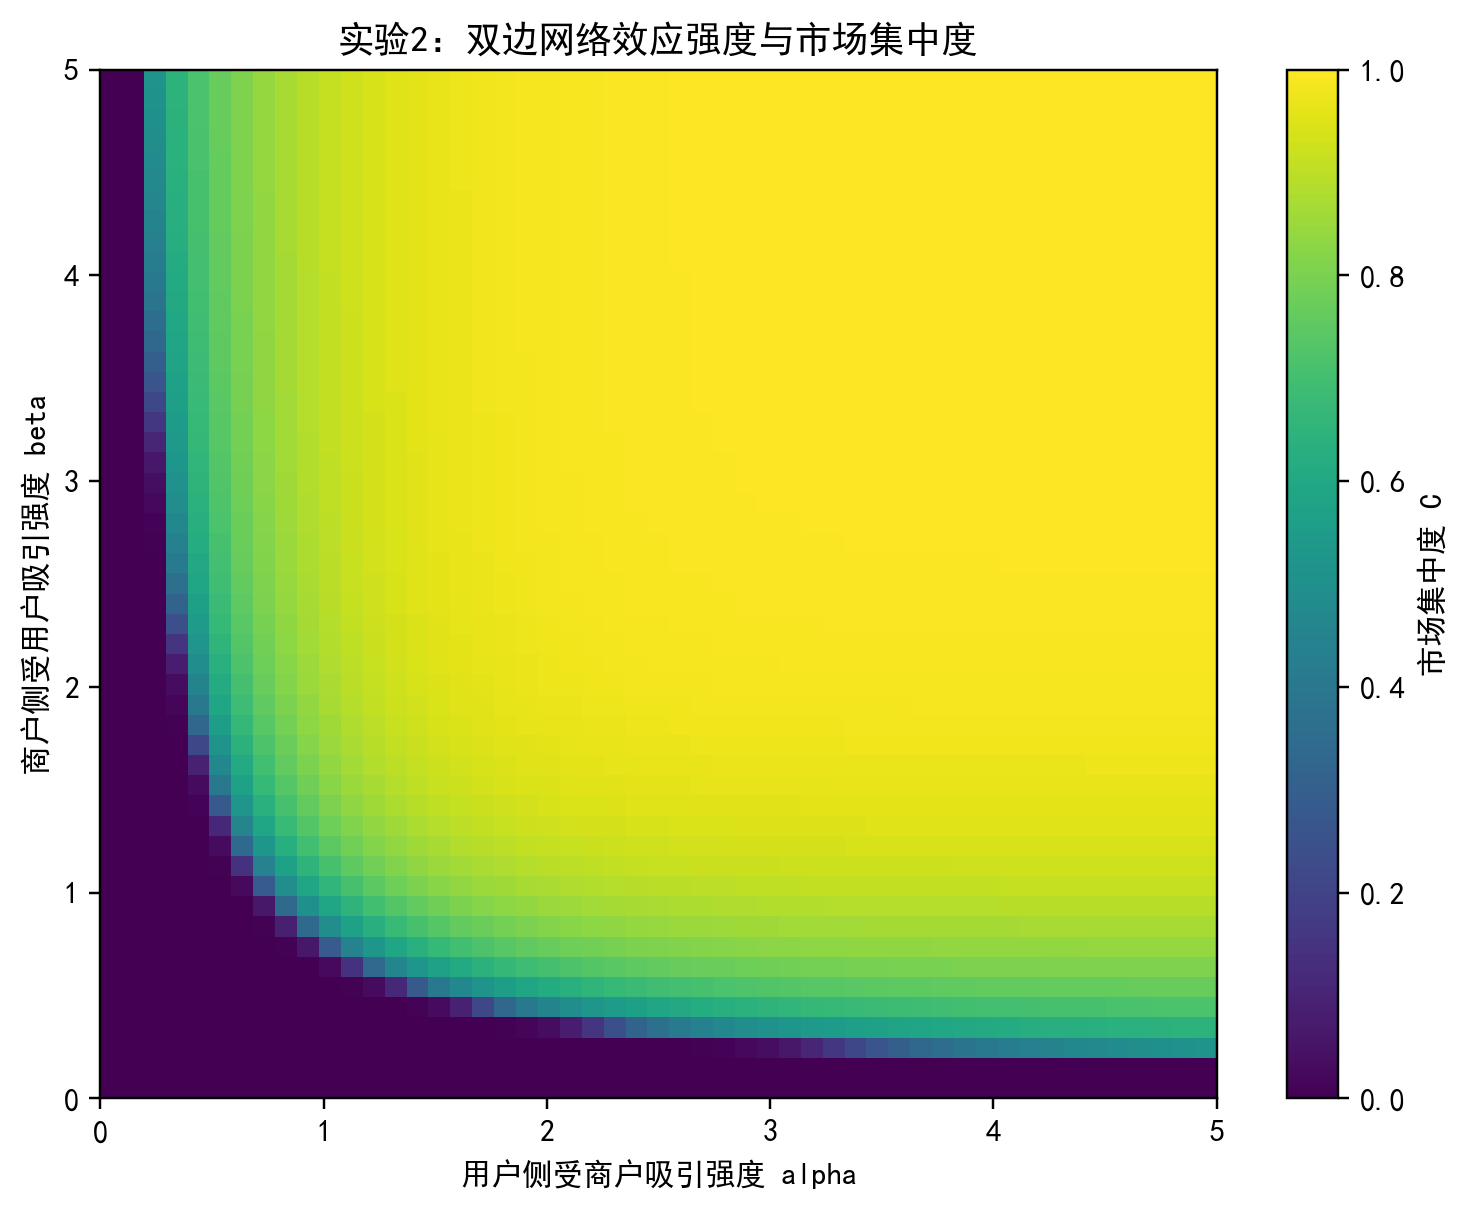
\includegraphics[width=\textwidth]{stage1_exp2_network.png}
    \caption{网络效应强度与集中度}
  \end{subfigure}
  \hfill
  \begin{subfigure}{0.49\textwidth}
    \centering
    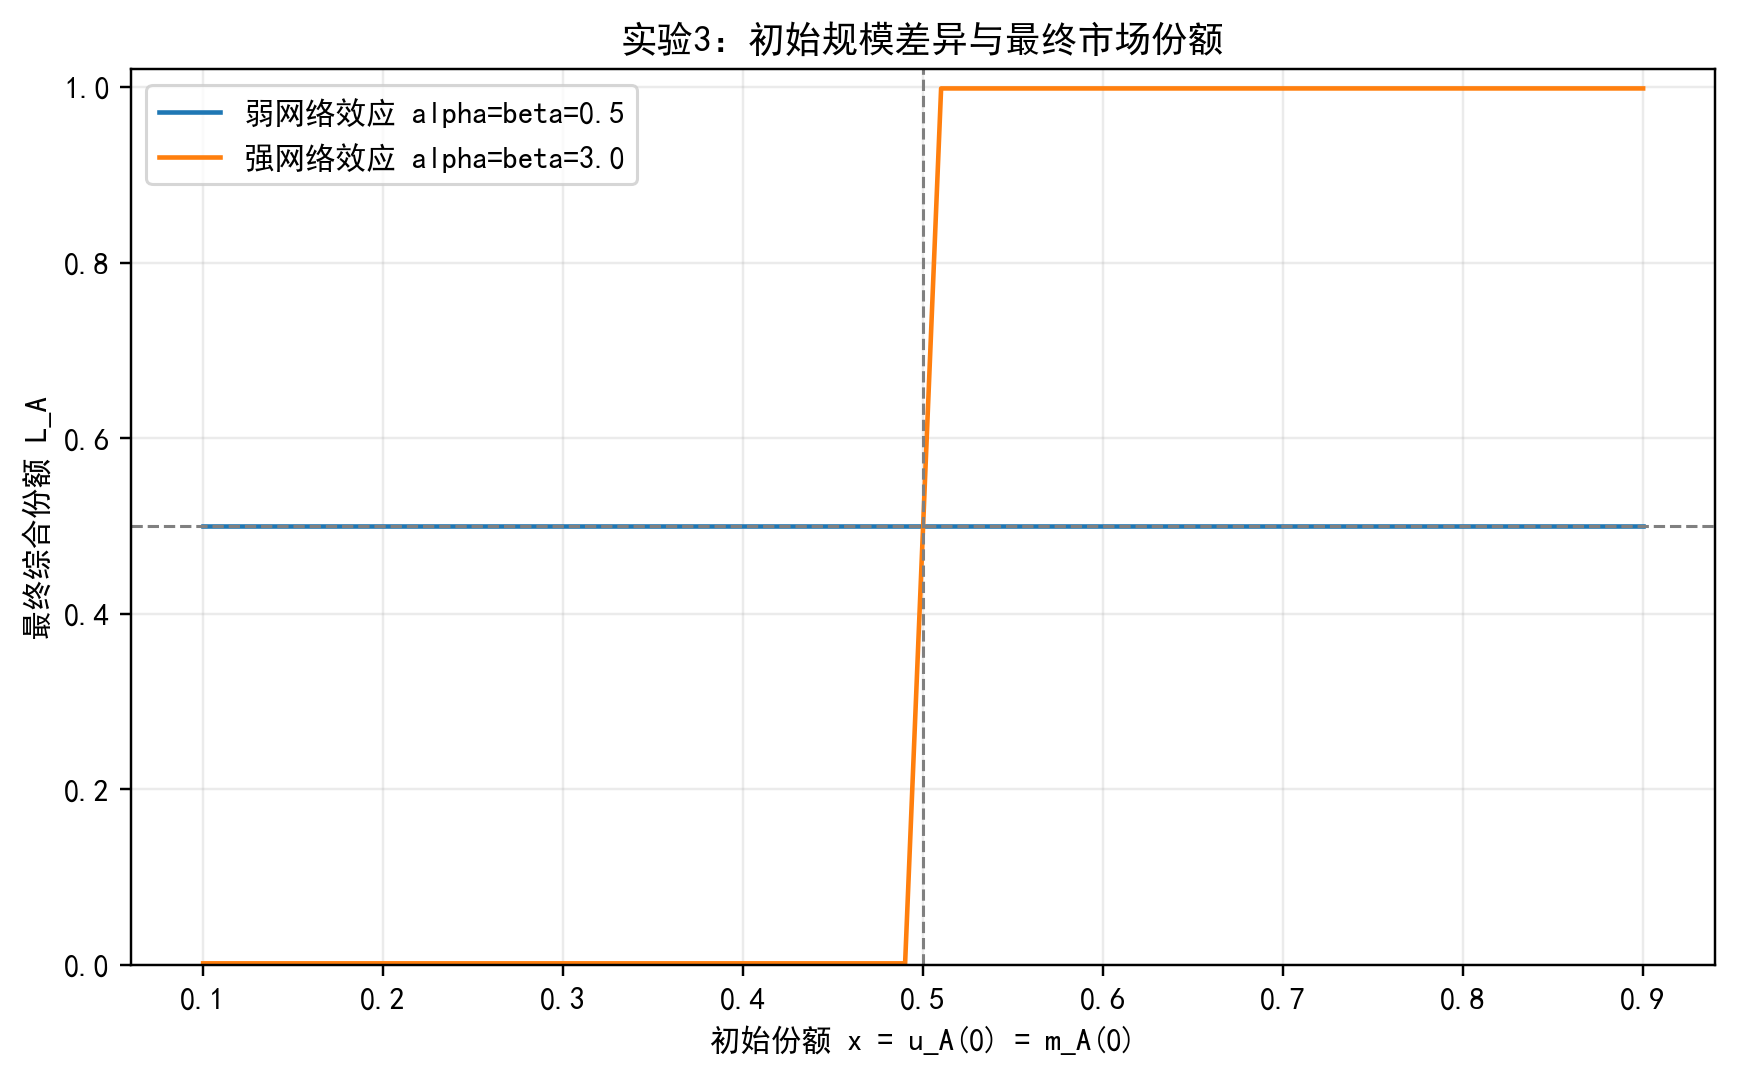
\includegraphics[width=\textwidth]{stage1_exp3_initial.png}
    \caption{初始份额与最终份额}
  \end{subfigure}
  \caption{阶段一实验 2--3：网络效应与初始优势}
  \label{fig:stage1-network-initial}
\end{figure}

实验 2 对 $\alpha,\beta\in[0,5]$ 进行二维扫描。结果显示，市场集中度随双边网络效应增强而上升。当 $\alpha$ 和 $\beta$ 都较弱时，平台更容易共存；当两侧网络效应同时较强时，初始小优势会被放大为长期锁定。值得注意的是，若只有一侧网络效应很强而另一侧为零，锁定并不稳定出现，说明赢家通吃不是单侧效应造成的，而是双边正反馈共同作用的结果。

实验 3 进一步说明初始规模差异的作用依赖网络效应强度。在弱网络效应下，不同初始份额最终趋向 $0.5$ 附近；在强网络效应下，初始份额略高于 $0.5$ 即可能导致平台 A 锁定，而略低于 $0.5$ 则可能导致平台 B 锁定。这表明平台竞争具有明显路径依赖，早期规模积累具有重要战略意义。

\subsection{服务质量和补贴干预}

\begin{figure}[H]
  \centering
  \begin{subfigure}{0.49\textwidth}
    \centering
    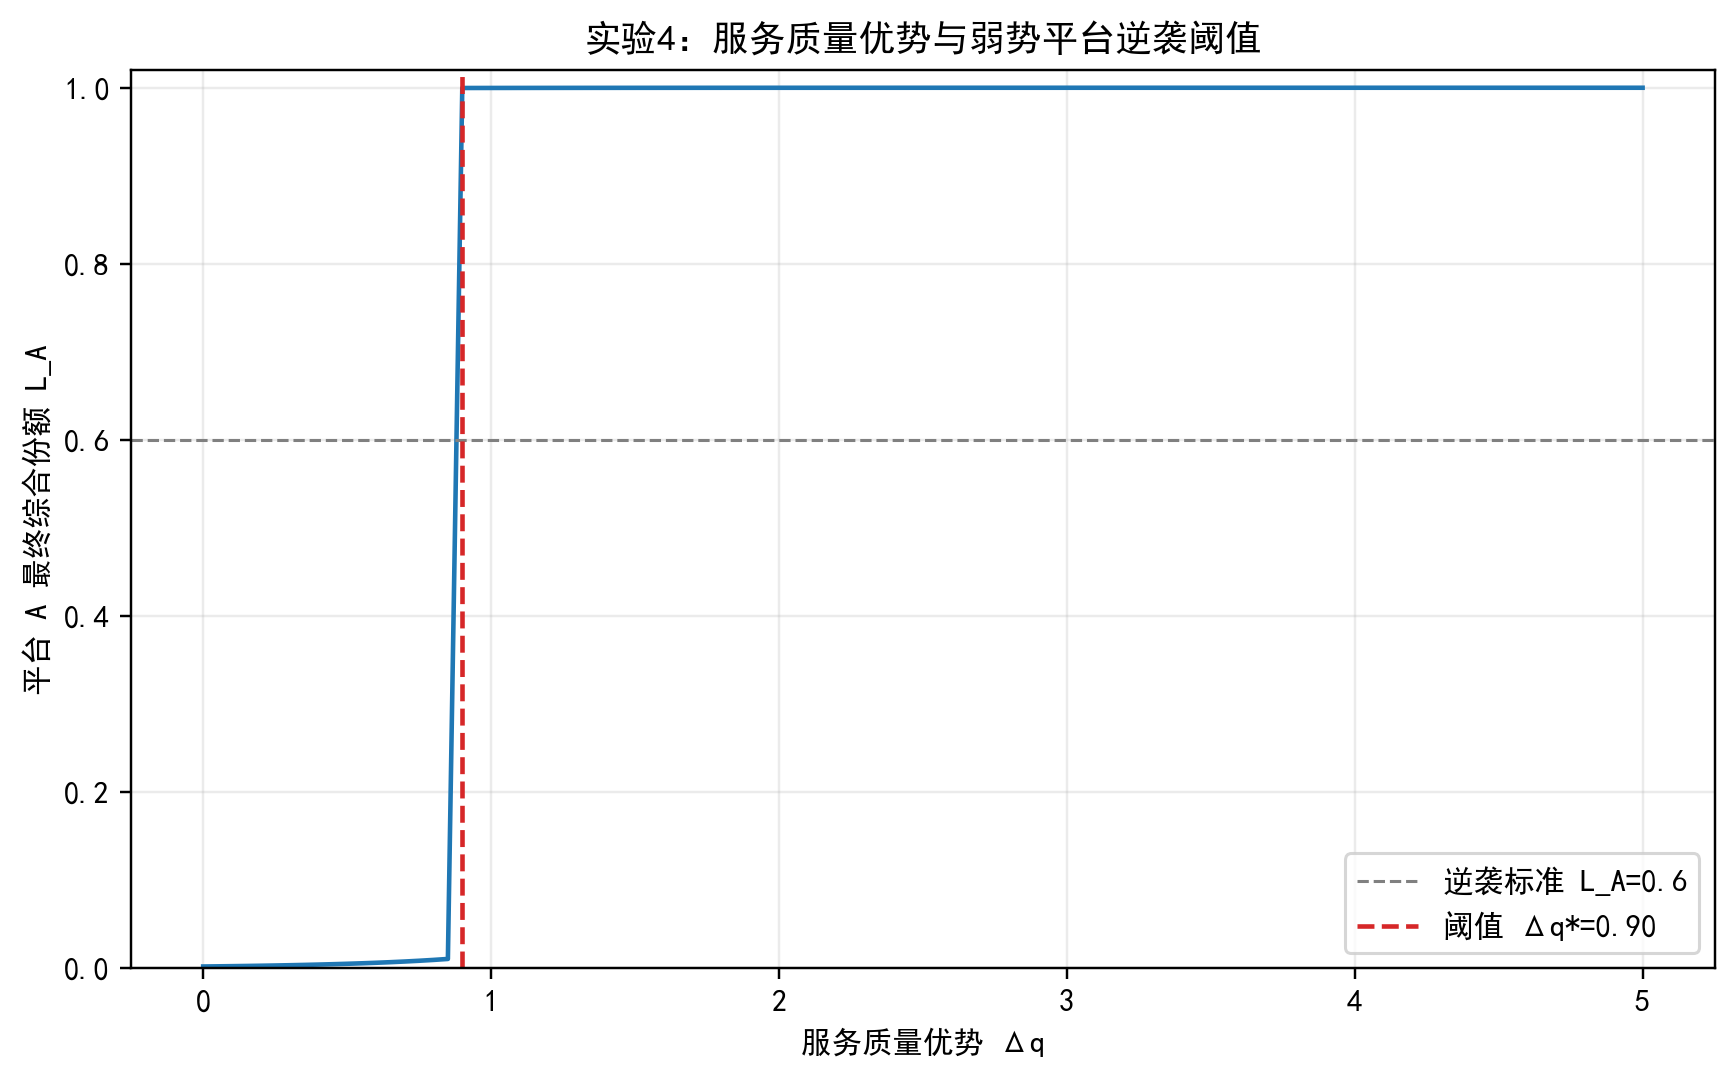
\includegraphics[width=\textwidth]{stage1_exp4_quality.png}
    \caption{服务质量优势阈值}
  \end{subfigure}
  \hfill
  \begin{subfigure}{0.49\textwidth}
    \centering
    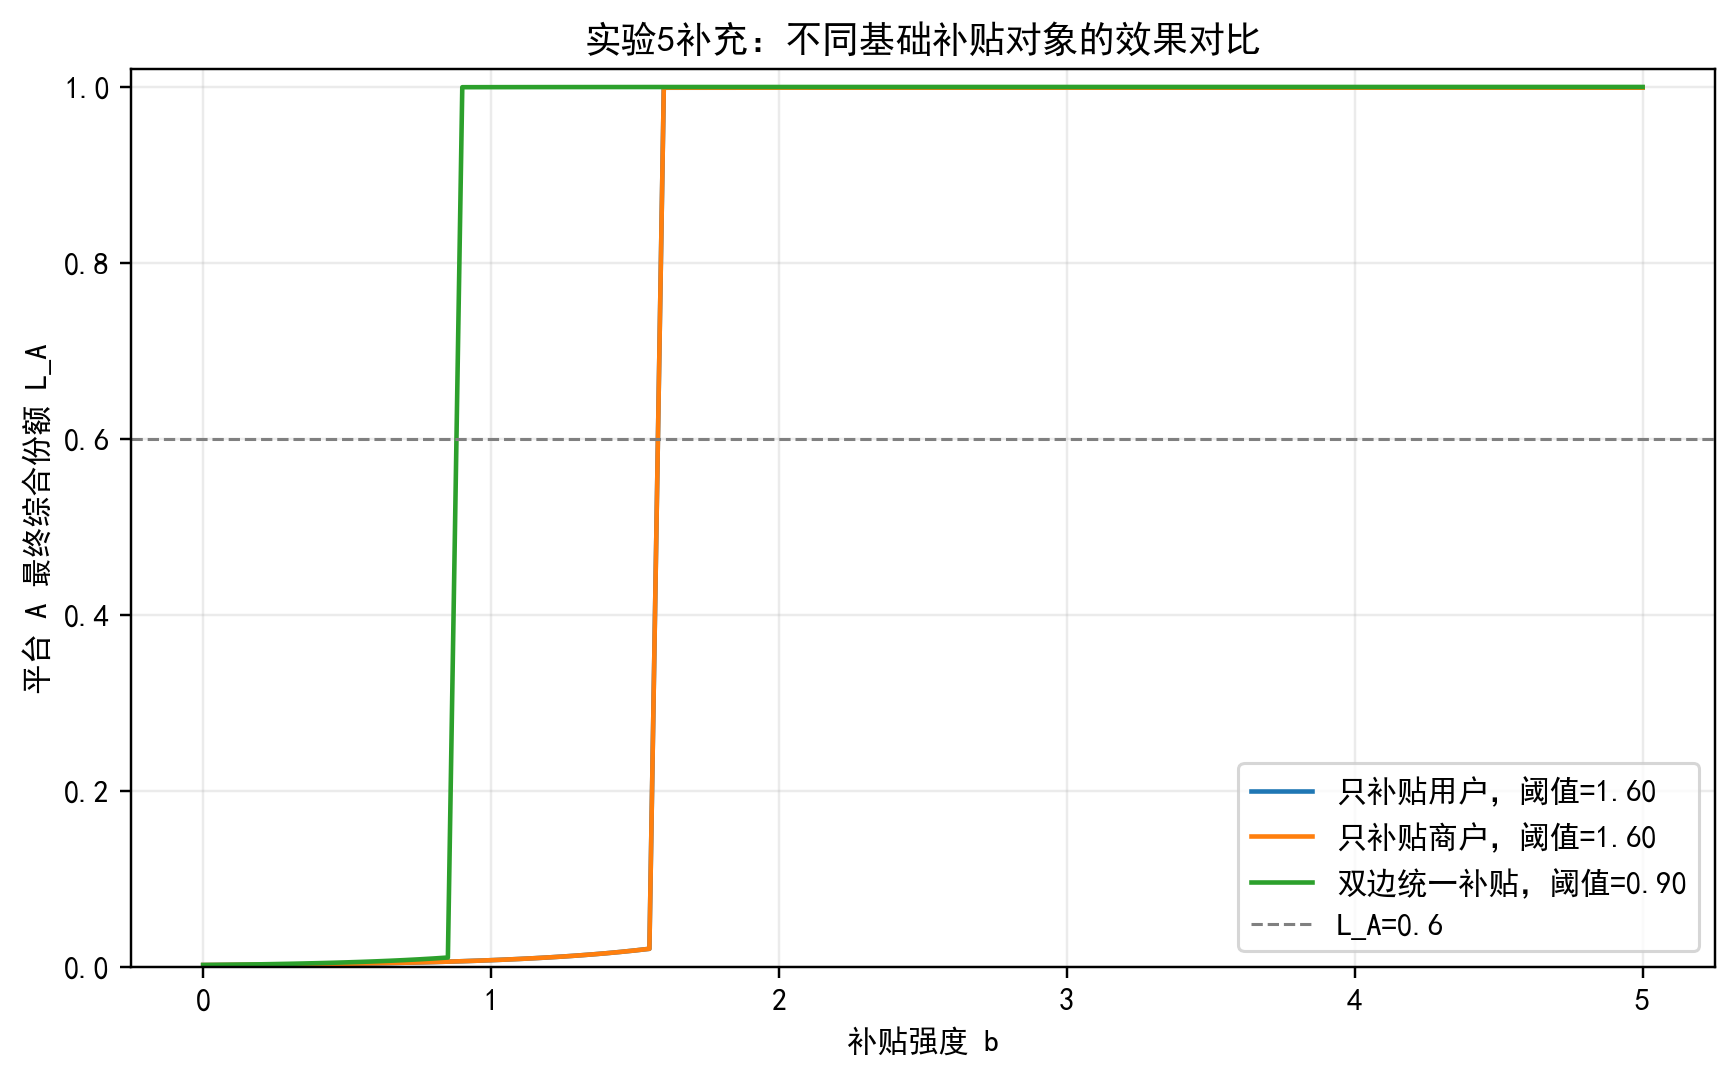
\includegraphics[width=\textwidth]{stage1_exp5_subsidy.png}
    \caption{不同补贴对象比较}
  \end{subfigure}
  \caption{阶段一实验 4--5：质量与补贴干预}
  \label{fig:stage1-quality-subsidy}
\end{figure}

实验 4 发现，弱势平台可以通过服务质量优势实现逆袭，但必须超过临界阈值。在强网络效应下，较小的质量优势不足以改变锁定格局；当服务质量优势达到约 $\Delta q^*=0.90$ 时，平台 A 才能快速跨越临界规模。实验 5 显示，统一双边补贴的突破阈值约为 $b^*=0.90$，而只补贴用户或只补贴商户需要更高强度，约为 $b=1.60$。这说明双边平台中单边刺激容易受另一侧规模不足限制，双边干预更容易形成正反馈。

\subsection{阶段一结论}

第一阶段验证了基础模型的合理性。双边平台竞争具有非线性、路径依赖和反馈放大特征。网络效应越强，初始规模优势越容易被放大；服务质量和补贴能够改变弱势平台地位，但都存在明确阈值。该阶段为后续临界区域识别和策略优化奠定了模型基础。

\section{第二阶段：临界条件与策略评估}

\subsection{市场状态区域与临界阈值}

第二阶段从“现象展示”转向“临界条件识别”。实验 6 将市场结果划分为共存、倾斜和锁定三类，并对 $\alpha,\beta$ 进行网格扫描。

\begin{figure}[H]
  \centering
  \begin{subfigure}{0.49\textwidth}
    \centering
    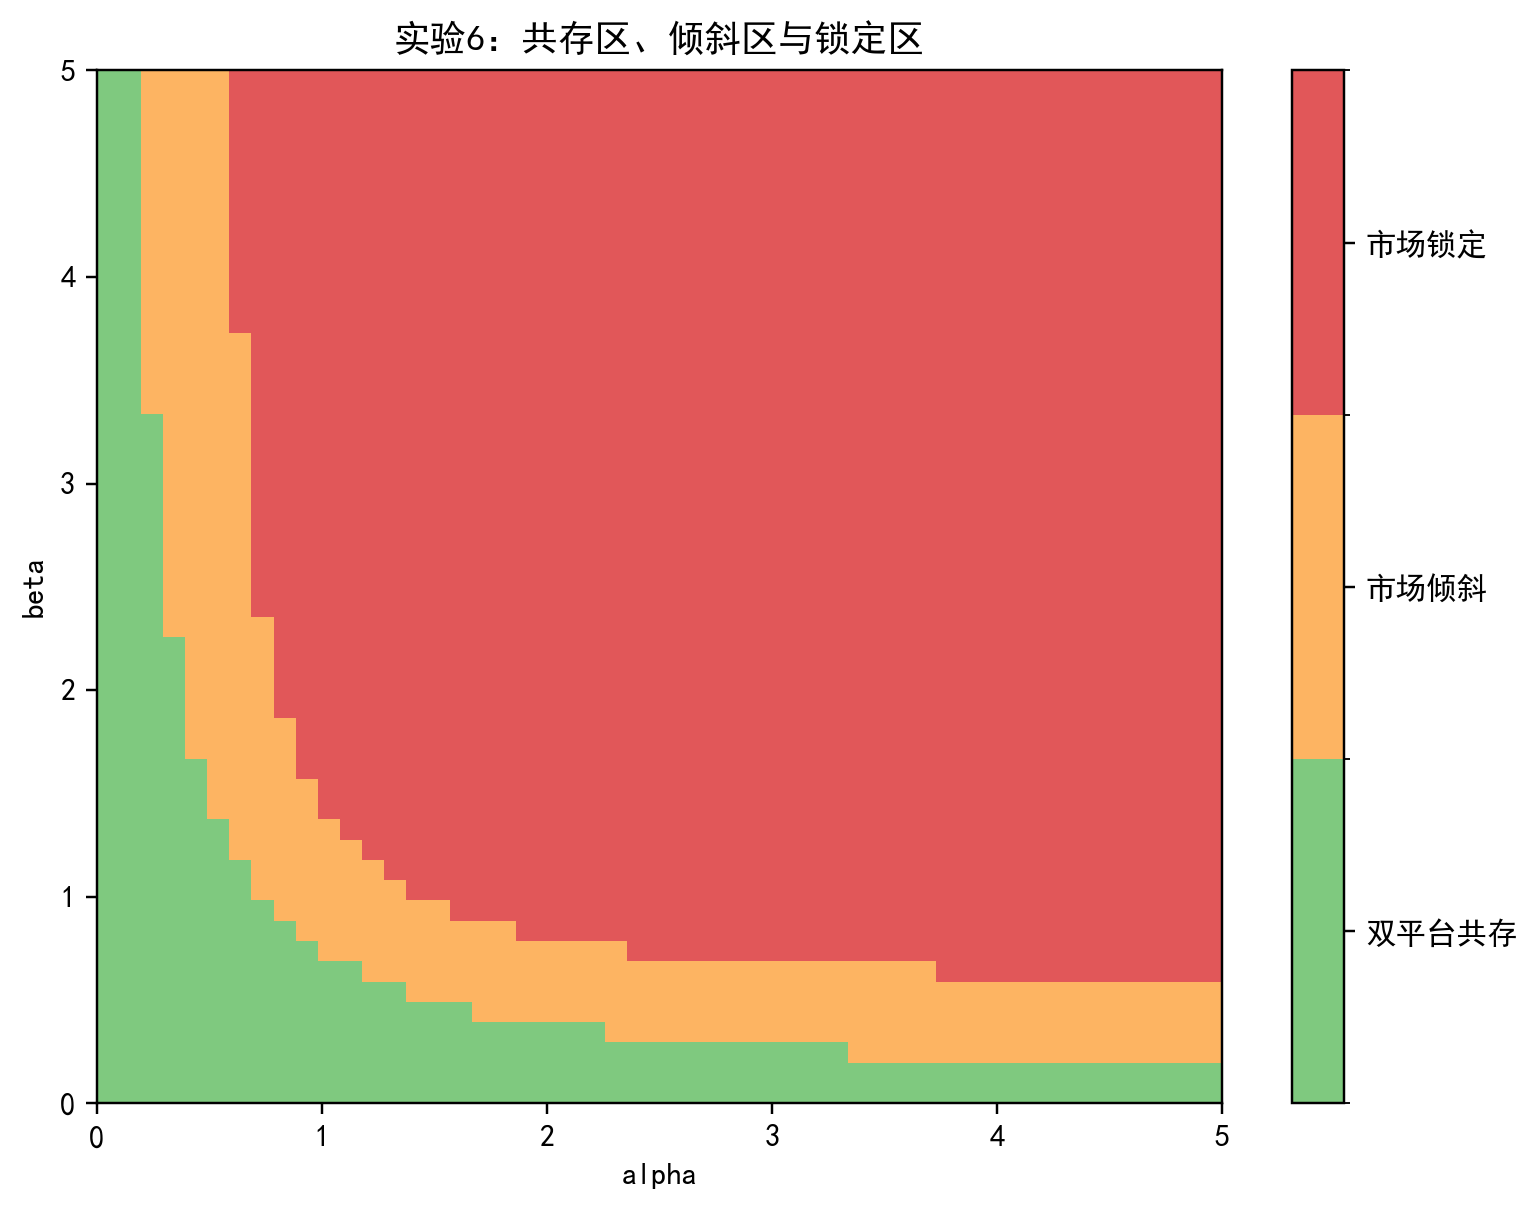
\includegraphics[width=\textwidth]{stage2_exp6_regions.png}
    \caption{市场状态分区}
  \end{subfigure}
  \hfill
  \begin{subfigure}{0.49\textwidth}
    \centering
    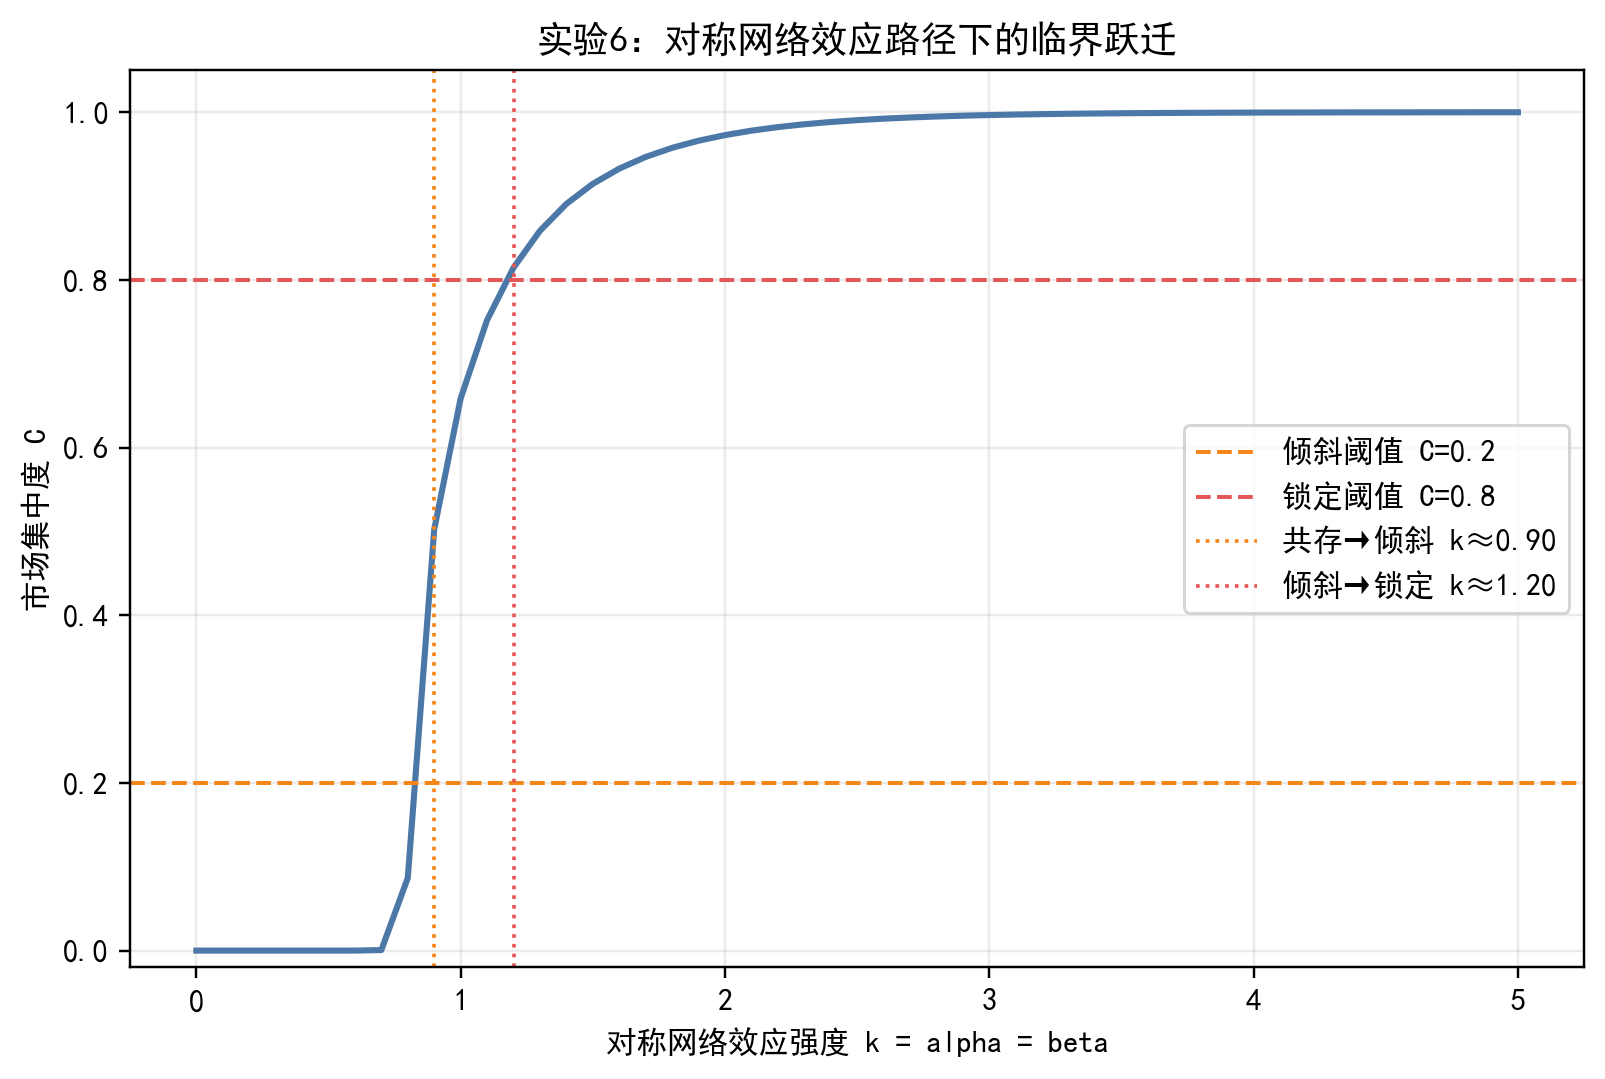
\includegraphics[width=\textwidth]{stage2_exp6_critical.png}
    \caption{对称网络效应路径}
  \end{subfigure}
  \caption{阶段二实验 6：市场锁定临界区域}
  \label{fig:stage2-regions}
\end{figure}

结果显示，在全部 2601 个参数组合中，共存区、倾斜区和锁定区均存在。沿 $\alpha=\beta=k$ 路径扫描时，共存到倾斜的阈值约为 $k_1^*\approx0.90$，倾斜到锁定的阈值约为 $k_2^*\approx1.20$。这说明市场结构变化不是平滑线性变化，而具有清晰阶段性。

\subsection{逆袭阈值与补贴分配}

\begin{figure}[H]
  \centering
  \begin{subfigure}{0.49\textwidth}
    \centering
    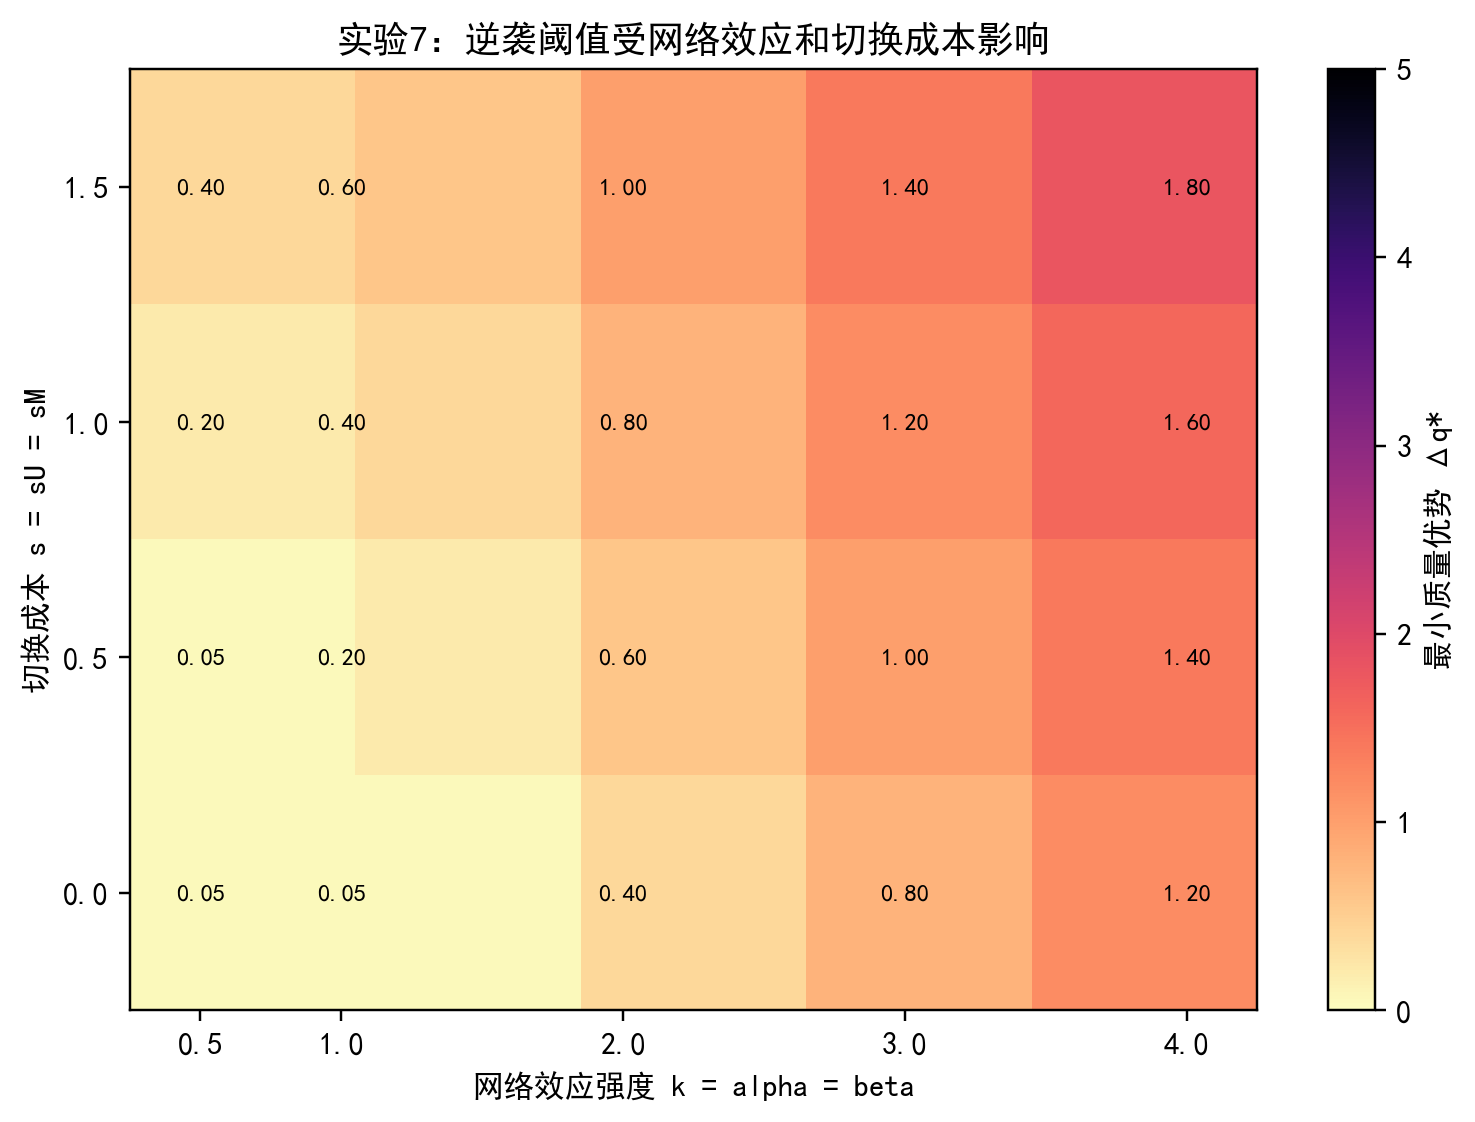
\includegraphics[width=\textwidth]{stage2_exp7_reversal.png}
    \caption{质量逆袭阈值}
  \end{subfigure}
  \hfill
  \begin{subfigure}{0.49\textwidth}
    \centering
    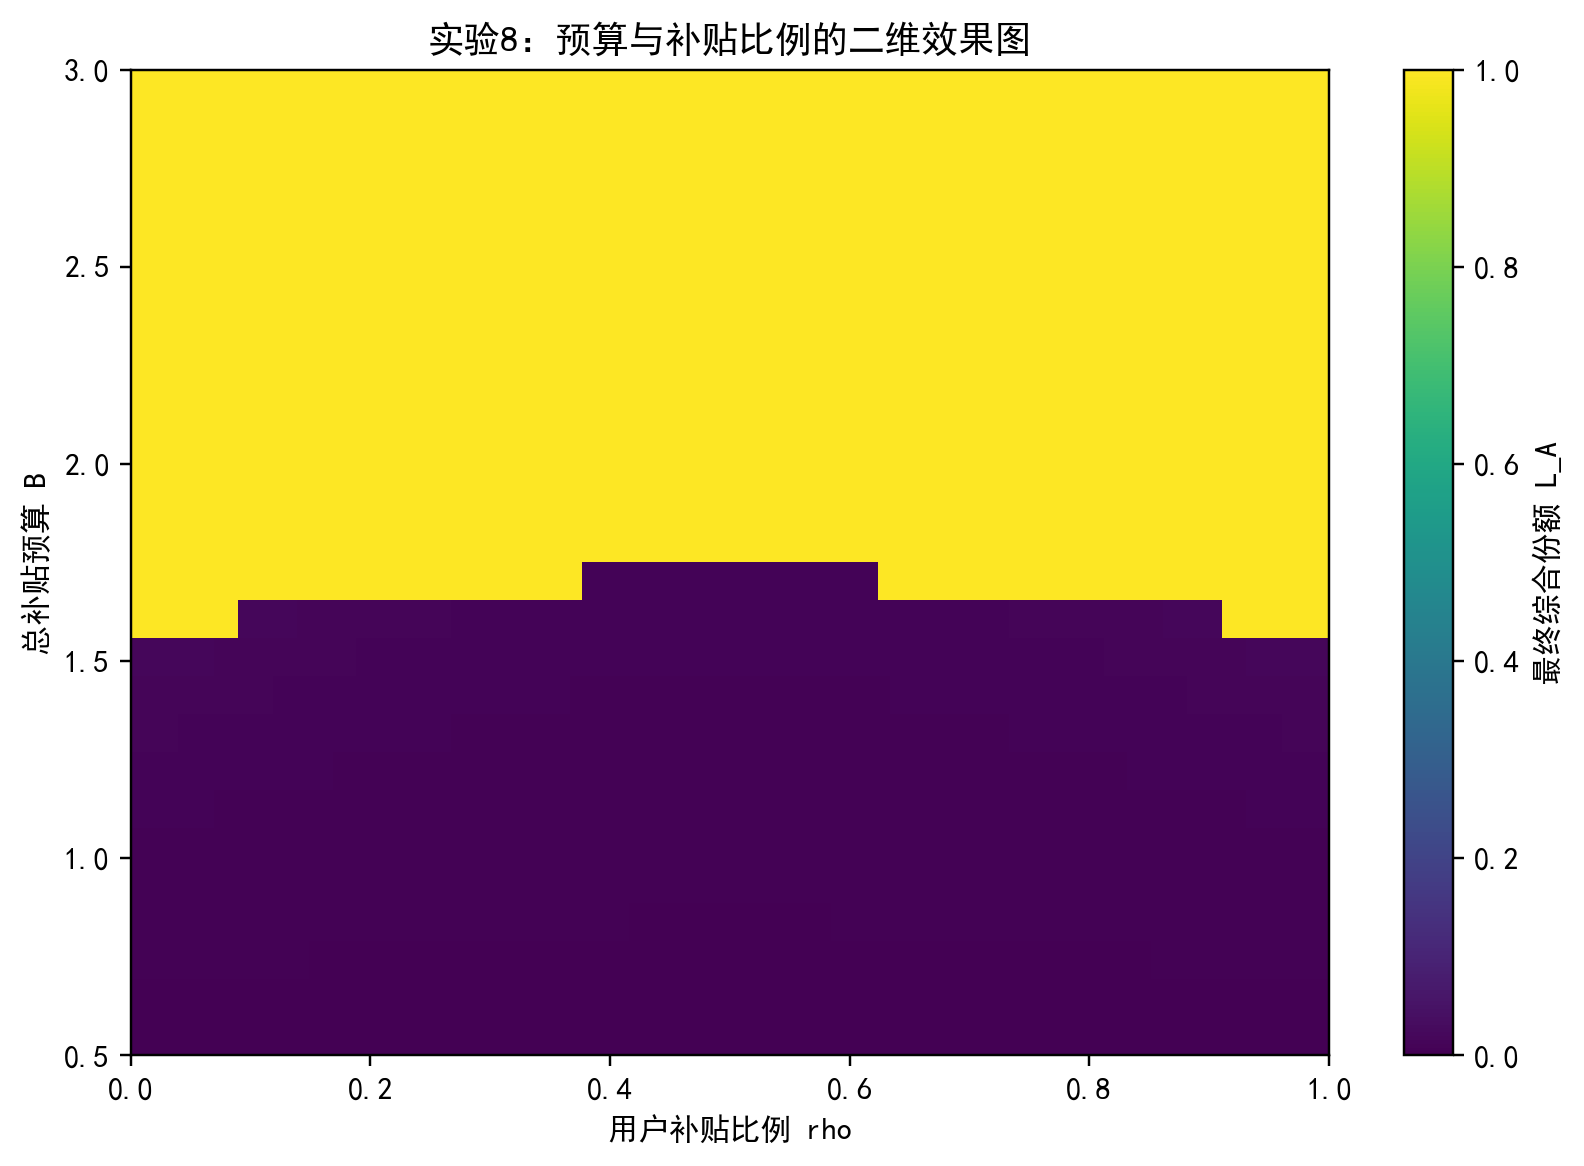
\includegraphics[width=\textwidth]{stage2_exp8_budget_rho.png}
    \caption{预算与补贴比例}
  \end{subfigure}
  \caption{阶段二实验 7--8：逆袭条件与补贴分配}
  \label{fig:stage2-reversal-subsidy}
\end{figure}

实验 7 发现，弱势平台逆袭所需服务质量优势随网络效应和切换成本共同上升。例如，当 $s=0$ 时，$k=0.5$ 或 $k=1.0$ 下只需很小质量优势即可逆袭；但当 $k=4.0$ 时，逆袭阈值升至约 $1.20$。切换成本提高后，同一网络效应强度下的逆袭阈值也显著上升。

实验 8 研究固定预算下的补贴分配。结果表明，预算不足时，无论如何分配都难以逆袭；预算达到临界区间后，补贴分配方式会显著影响结果。对称网络效应下，当预算足够时双边均衡补贴更稳定；非对称网络效应下，应优先补贴更能触发另一侧加入的一边。例如用户更依赖商户规模时，应优先补贴商户；商户更依赖用户规模时，应优先补贴用户。

\subsection{补贴退出与利润约束}

\begin{figure}[H]
  \centering
  \begin{subfigure}{0.49\textwidth}
    \centering
    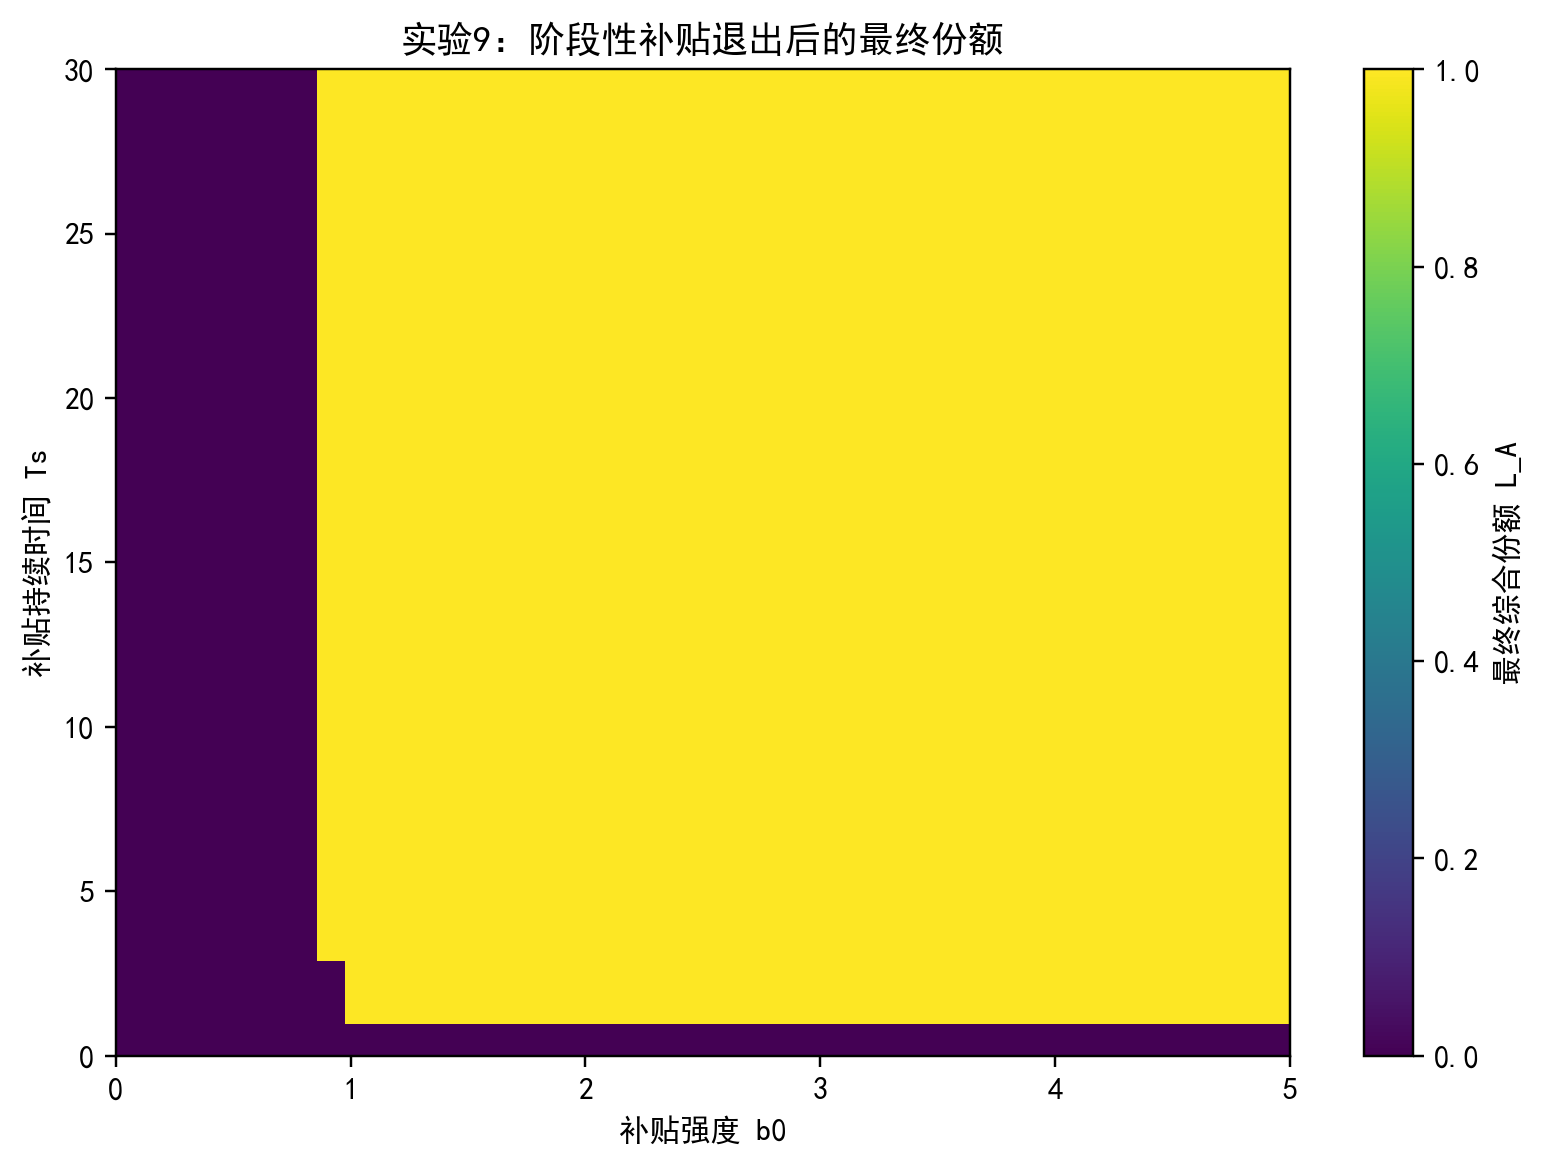
\includegraphics[width=\textwidth]{stage2_exp9_exit.png}
    \caption{阶段性补贴退出}
  \end{subfigure}
  \hfill
  \begin{subfigure}{0.49\textwidth}
    \centering
    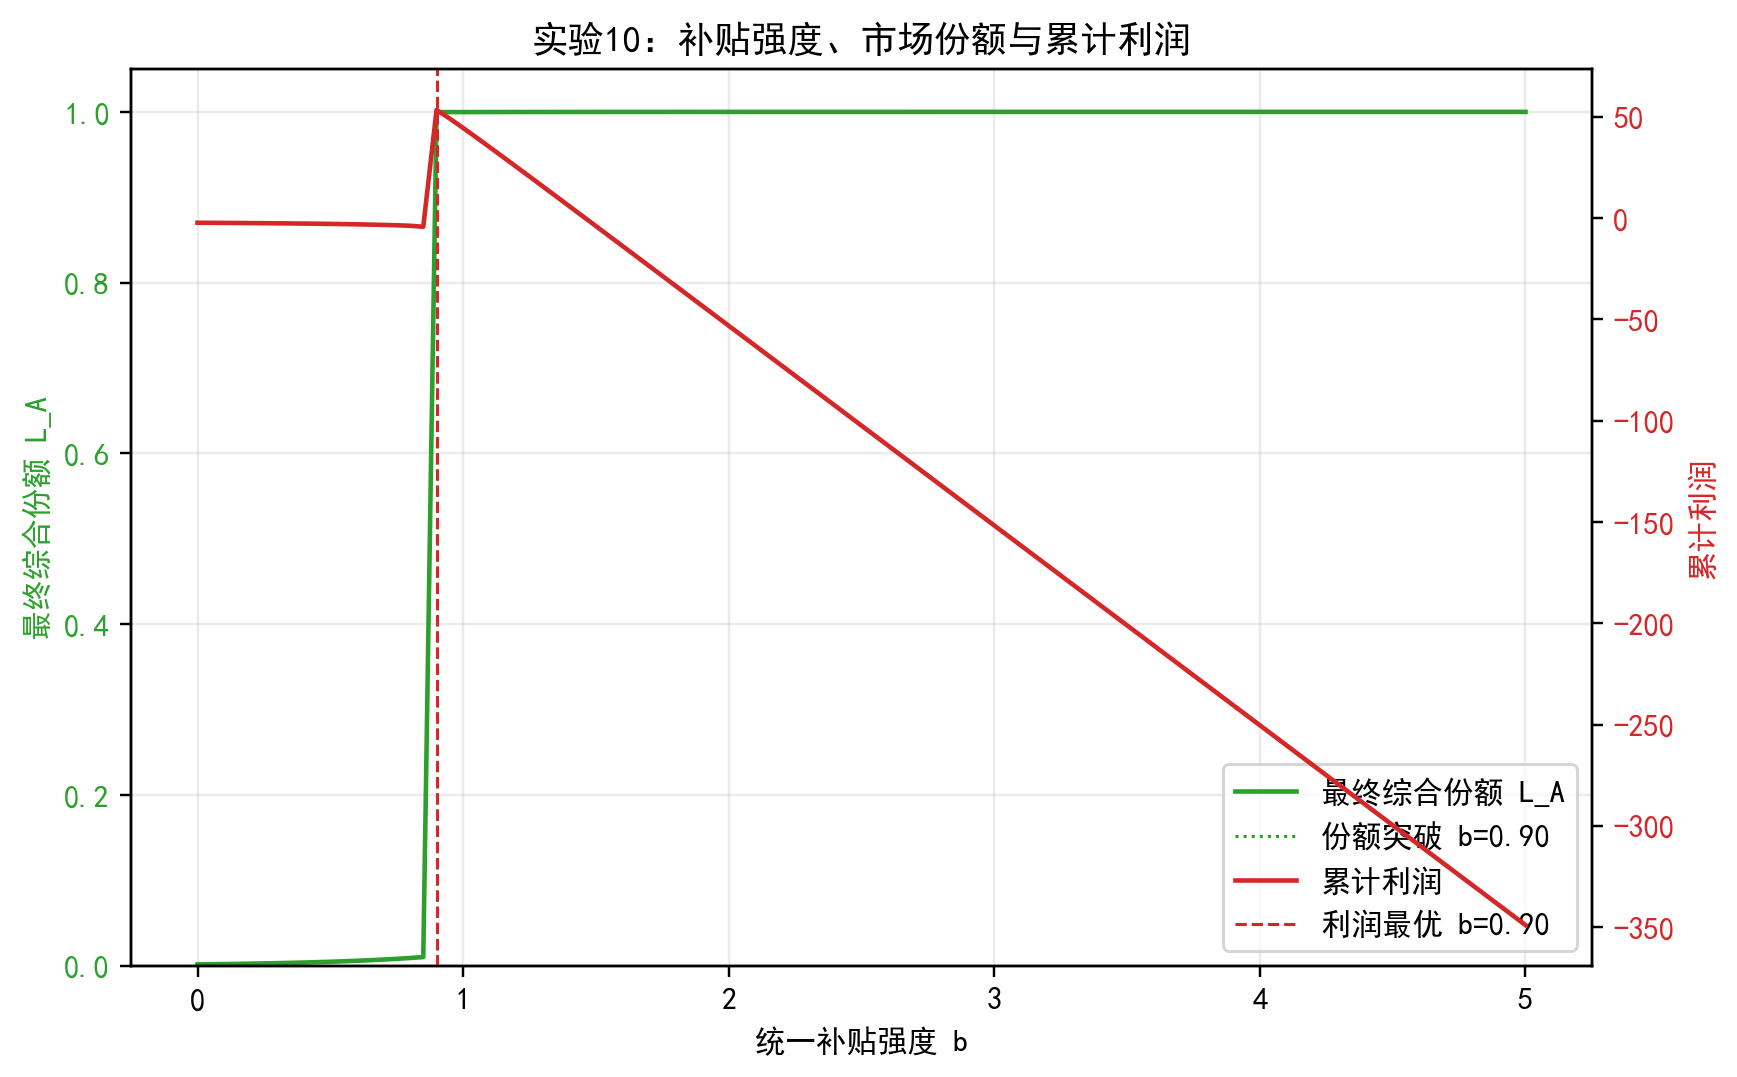
\includegraphics[width=\textwidth]{stage2_exp10_profit.png}
    \caption{补贴强度与利润}
  \end{subfigure}
  \caption{阶段二实验 9--10：补贴持续时间与经济可行性}
  \label{fig:stage2-exit-profit}
\end{figure}

实验 9 显示，补贴不必永久持续。只要补贴强度和持续时间足以帮助平台跨过临界规模，补贴退出后平台仍可依靠已形成的双边网络效应维持优势。实验 10 进一步纳入利润约束，发现市场份额和利润并不总是同向变化。低补贴无法突破锁定，过高补贴虽然保持高份额但成本过大；在本实验中，$b=0.90$ 附近既能跨越临界规模，又能获得较高累计利润。

\subsection{阶段二结论}

第二阶段说明，平台策略的核心不是简单提高网络效应、服务质量或补贴总量，而是识别并跨越临界条件。网络效应、切换成本、质量优势和补贴策略之间存在复杂交互。平台应围绕“跨越临界规模”设计阶段性、结构化干预，而不是追求短期份额或补贴强度最大化。

\section{第三阶段：ABM 多智能体机制实验}

\subsection{ABM 模型扩展}

前两阶段的 ODE 模型描述平均份额演化，适合刻画宏观趋势，但难以表达个体异质性、随机选择、精准补贴和多归属行为。因此第三阶段使用 Mesa 框架构建 Agent-Based Model \cite{kazil2020,wilensky2015}。模型将用户和商户表示为 agent，每个主体具有价格敏感度、补贴敏感度、惯性、质量偏好和随机扰动。商户可处于 A-only、B-only 或 multi-home 状态。ABM 的目标不是替代 ODE，而是检验并扩展前两阶段机制结论。

\subsection{个体异质性与精准补贴}

\begin{figure}[H]
  \centering
  \begin{subfigure}{0.49\textwidth}
    \centering
    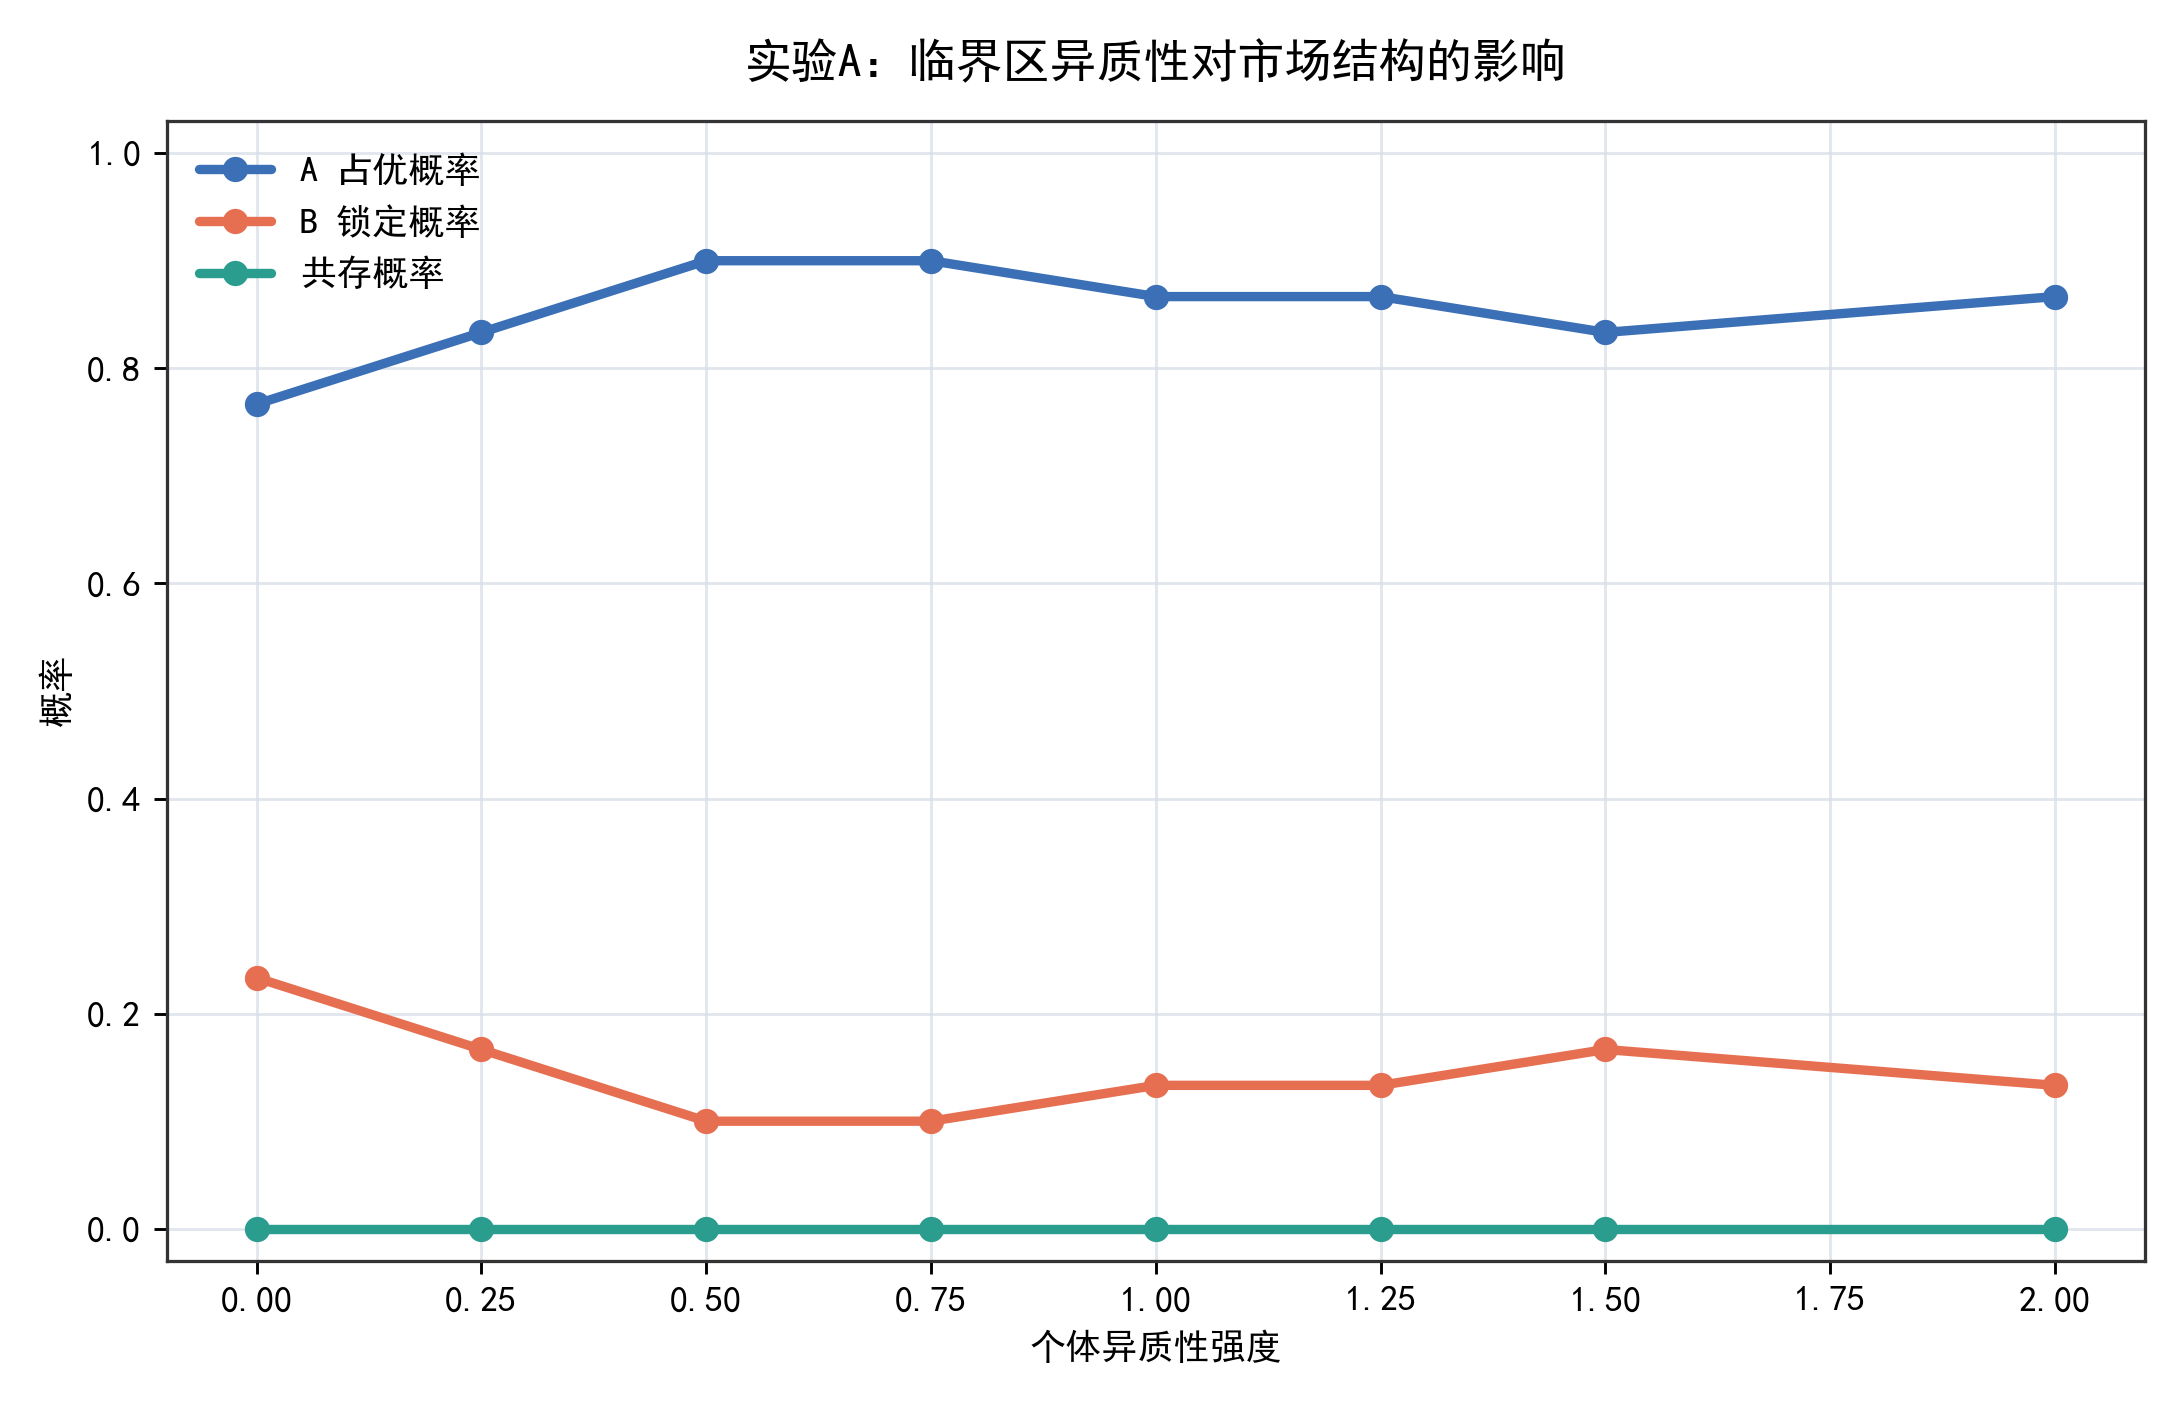
\includegraphics[width=\textwidth]{abm_a_heterogeneity.png}
    \caption{异质性与市场结构}
  \end{subfigure}
  \hfill
  \begin{subfigure}{0.49\textwidth}
    \centering
    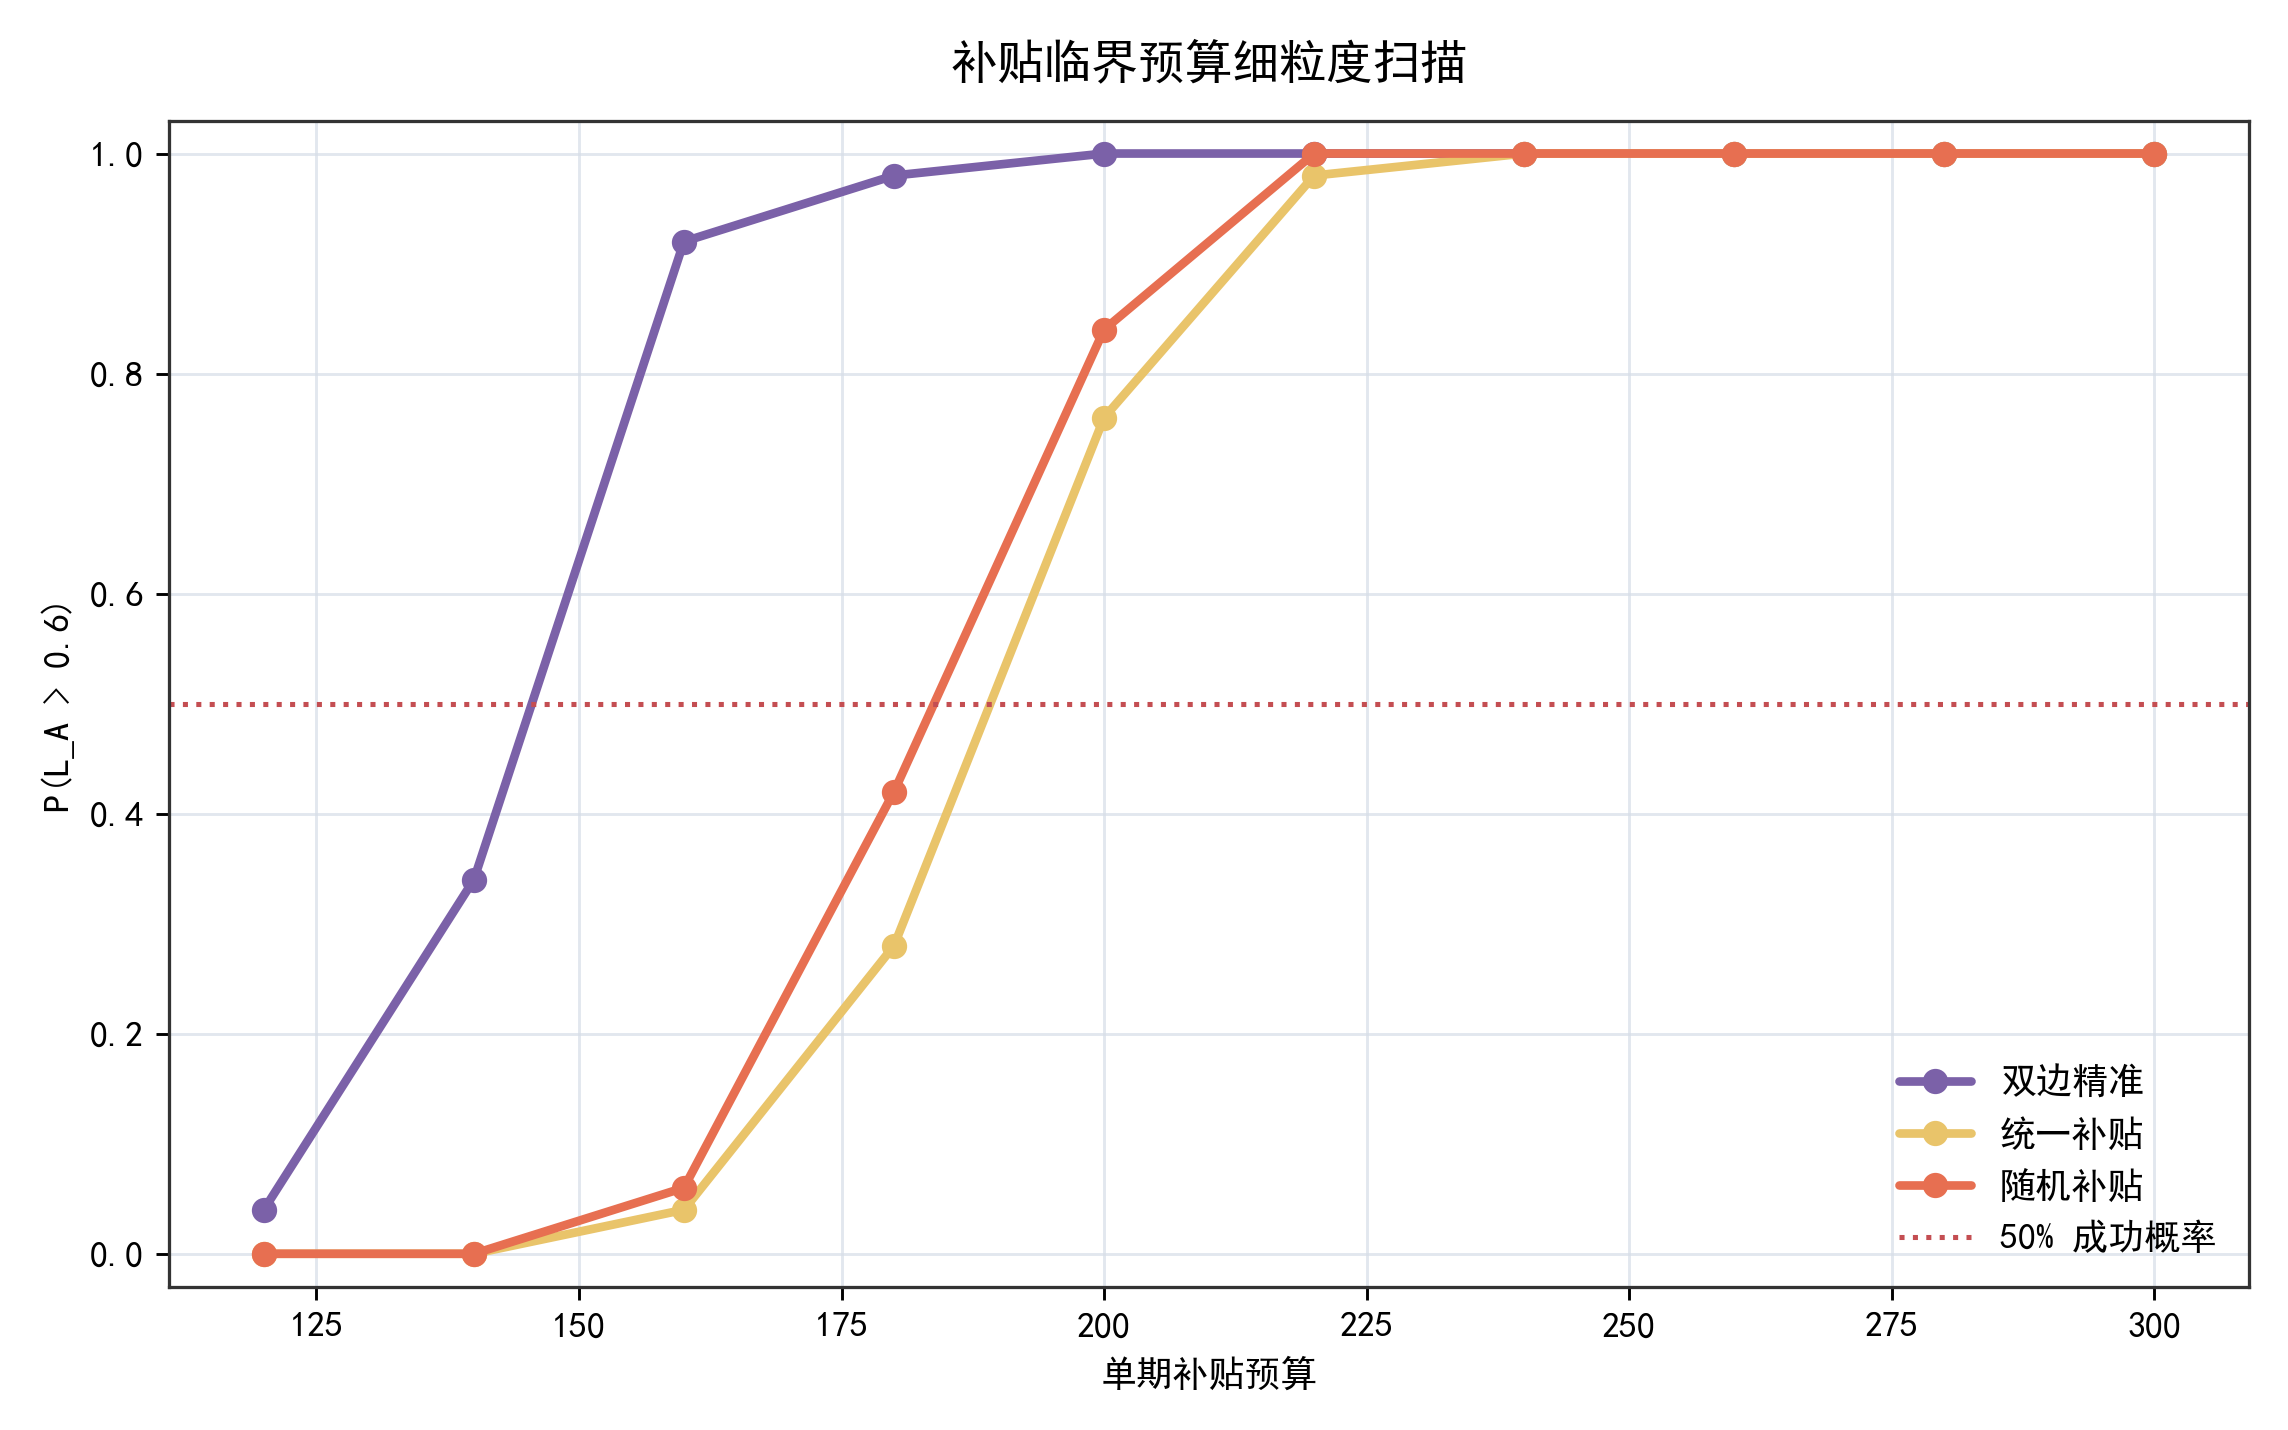
\includegraphics[width=\textwidth]{abm_b_budget.png}
    \caption{细粒度临界预算}
  \end{subfigure}
  \caption{阶段三实验 A--B：异质性与补贴策略}
  \label{fig:abm-ab}
\end{figure}

实验 A 表明，个体异质性的作用并非单调。中等异质性可能使部分高敏感主体率先响应初始优势，从而强化领先平台的正反馈；强异质性则可能降低市场集中度，使不同偏好的用户和商户保留在不同平台。实验 B 在等预算下比较统一补贴、随机补贴和双边精准补贴。细粒度扫描显示，双边精准补贴的临界预算约为 160，而统一补贴和随机补贴约为 200。这说明 ABM 下补贴效率取决于投向对象，而不只是预算总量。

\subsection{冷启动与多归属机制}

\begin{figure}[H]
  \centering
  \begin{subfigure}{0.49\textwidth}
    \centering
    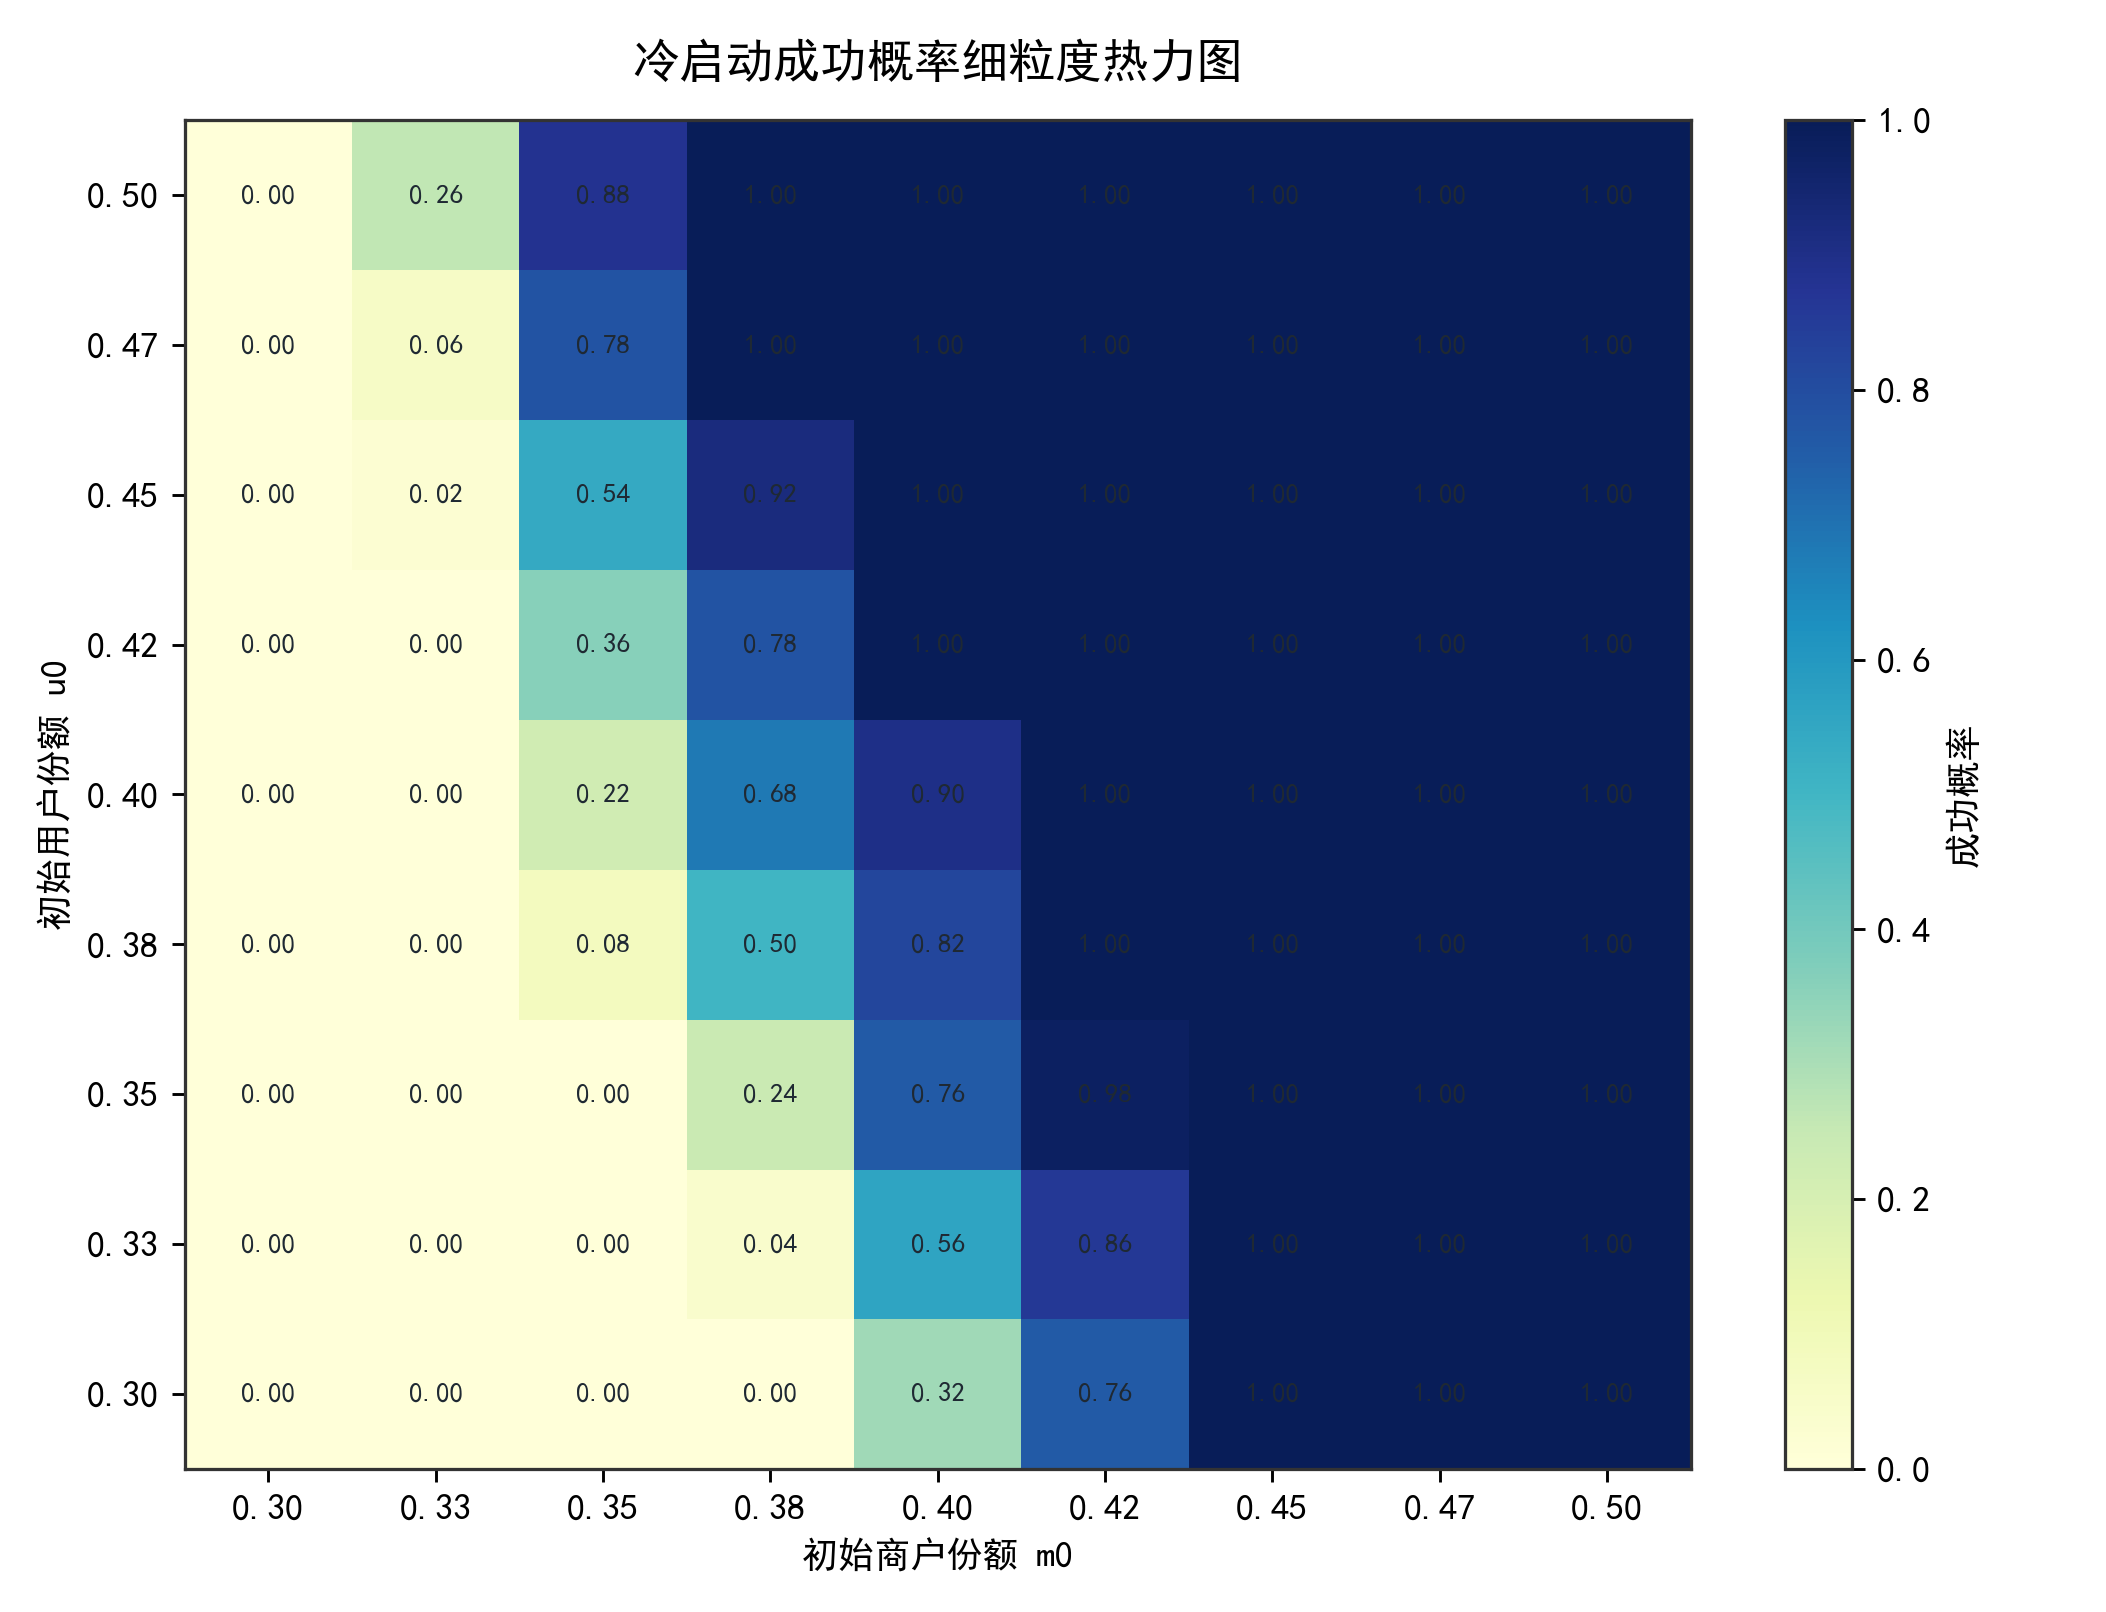
\includegraphics[width=\textwidth]{abm_c_cold_start.png}
    \caption{冷启动成功概率}
  \end{subfigure}
  \hfill
  \begin{subfigure}{0.49\textwidth}
    \centering
    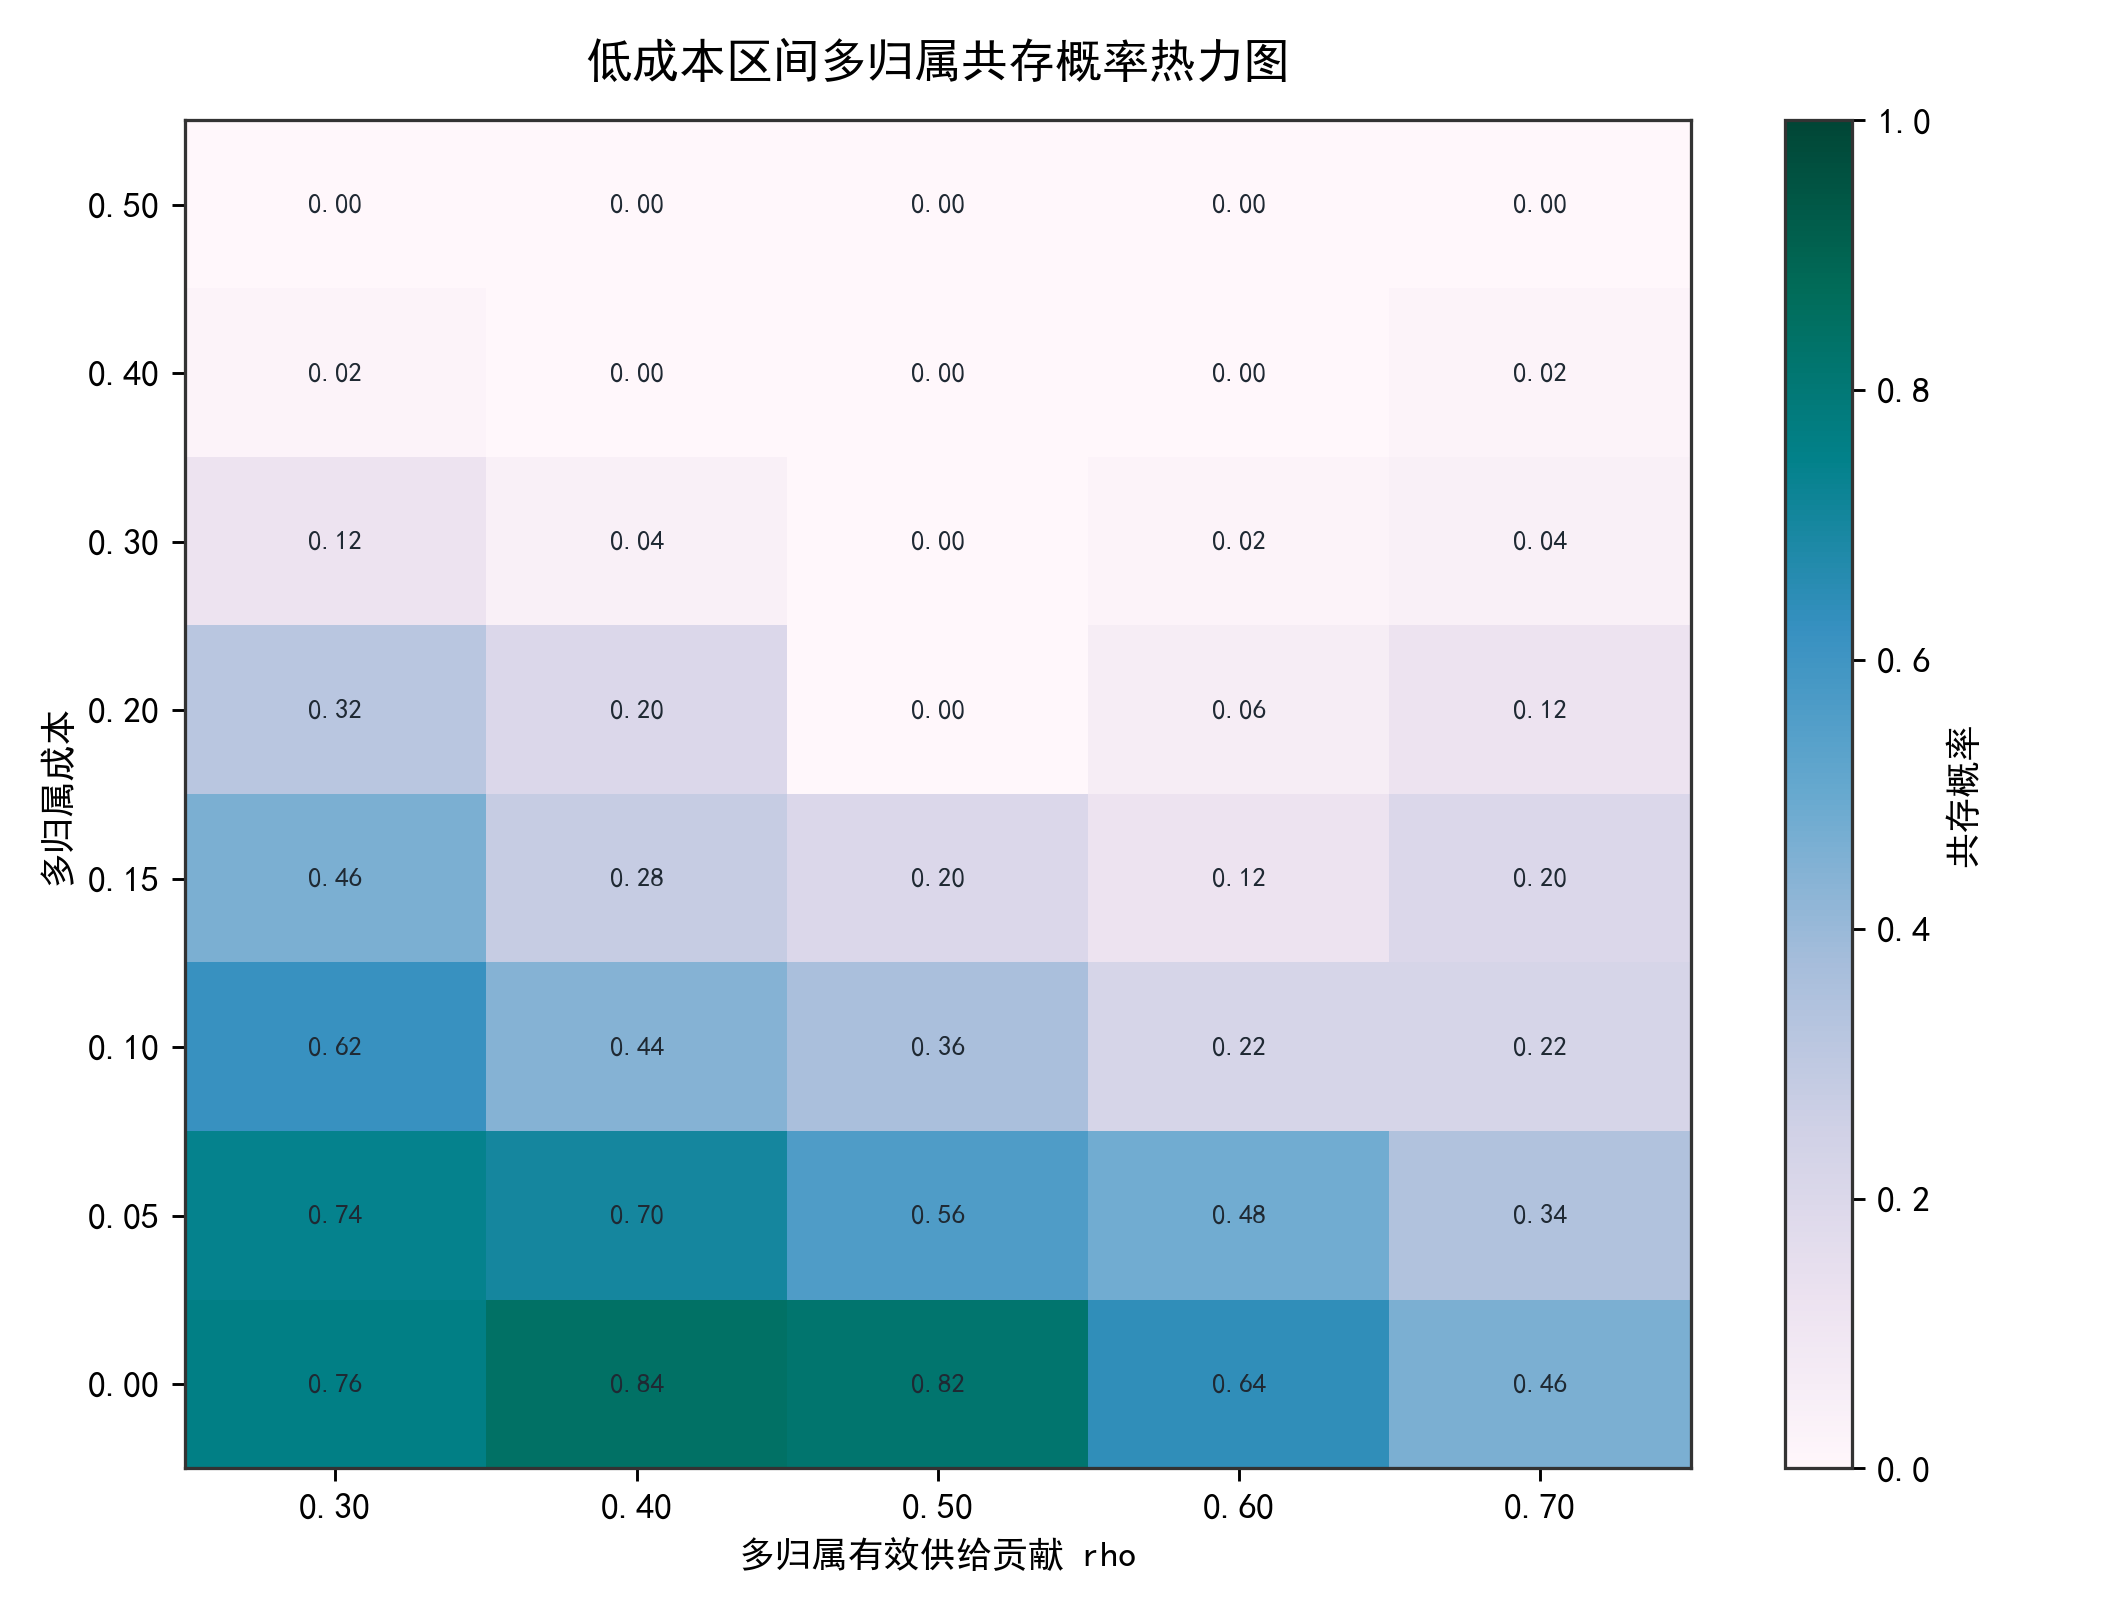
\includegraphics[width=\textwidth]{abm_d_multihome.png}
    \caption{多归属共存概率}
  \end{subfigure}
  \caption{阶段三实验 C--D：冷启动与商户多归属}
  \label{fig:abm-cd}
\end{figure}

冷启动实验显示，平台成功区域主要位于用户侧和商户侧初始资源同时较高的区域。商户初始份额过低时，即使提高用户初始份额，平台也难以触发正反馈；商户供给达到一定水平后，用户侧资源的边际作用才明显增强。多归属实验显示，低成本多归属有助于平台共存；当多归属成本升高后，商户重新转向单一平台，市场更容易锁定。

\begin{figure}[H]
  \centering
  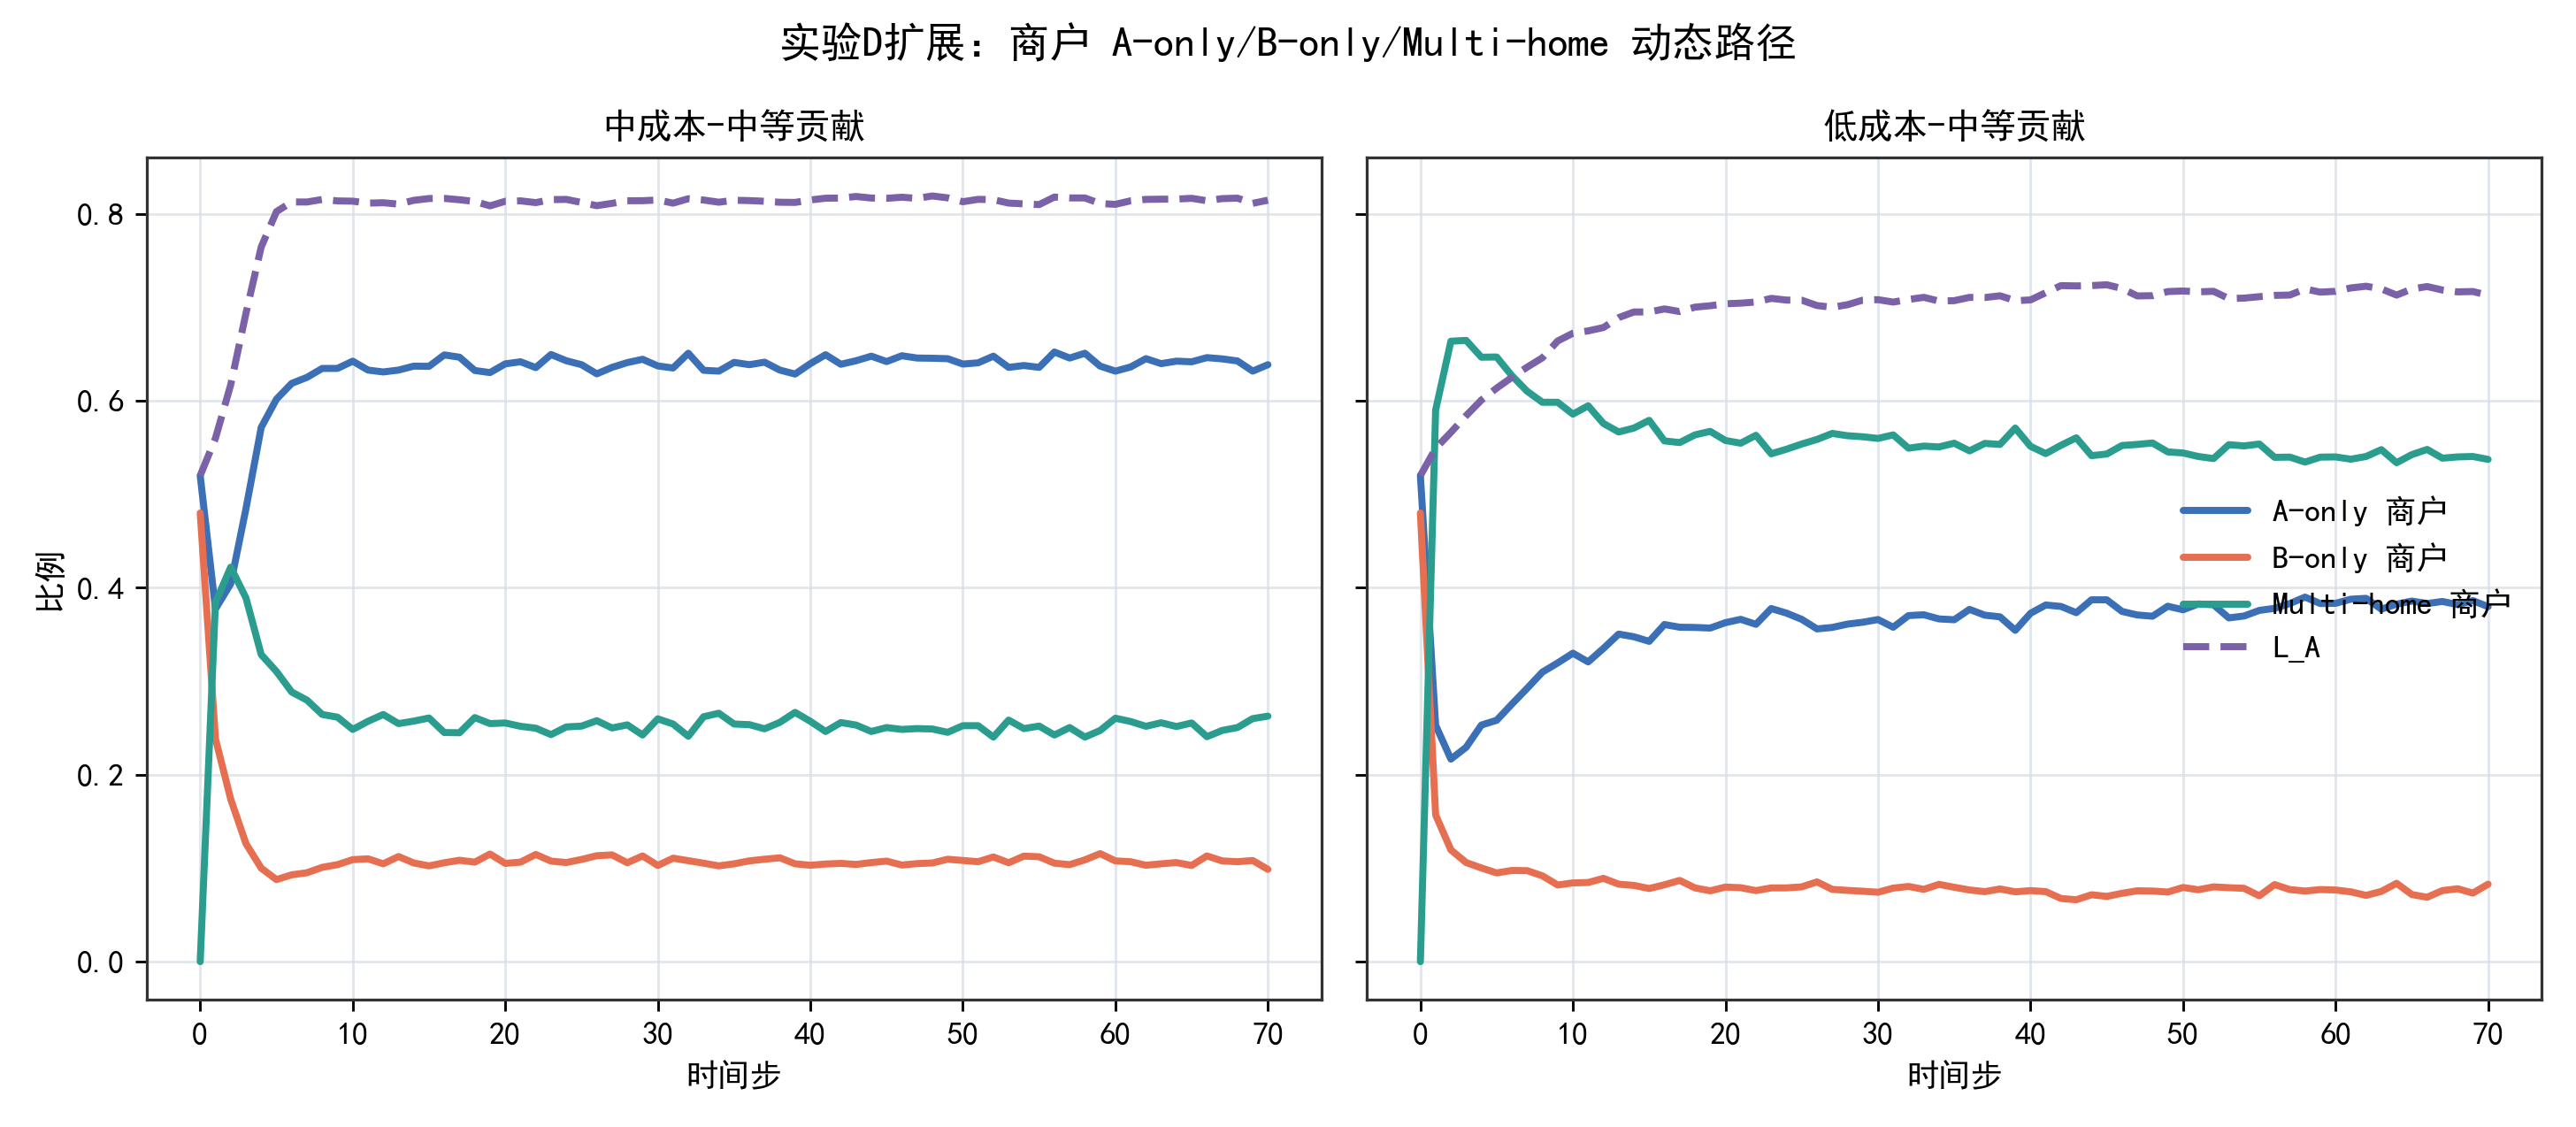
\includegraphics[width=0.86\textwidth]{abm_d_paths.png}
  \caption{商户 A-only、B-only 与 multi-home 动态路径}
  \label{fig:abm-paths}
\end{figure}

图 \ref{fig:abm-paths} 进一步展示了多归属的动态机制。低成本场景下，multi-home 商户可长期保持较高比例，从而缓和两平台间供给差异；高成本场景下，商户迅速转向单一平台，供给侧差异被放大，市场更容易出现锁定。

\subsection{机制消融与 ODE 对比}

为进一步检验 ABM 结论是否确由模型机制驱动，本文补充机制消融实验。实验在弱势平台补贴临界区设定 $u_A(0)=m_A(0)=0.30$、$B=140$，逐一去掉个体异质性、惯性、精准补贴规则、多归属和双边网络效应。结果显示，去掉双边网络效应后，平台 A 成功概率降至 0.10，A 锁定概率为 0；去掉商户多归属后，成功概率降至 0.30，最终份额波动显著增大。这说明补贴能否发挥作用，关键取决于其是否被双边网络效应放大，以及商户多归属是否能为弱势平台提供启动期供给缓冲。

\begin{figure}[H]
  \centering
  \begin{subfigure}{0.49\textwidth}
    \centering
    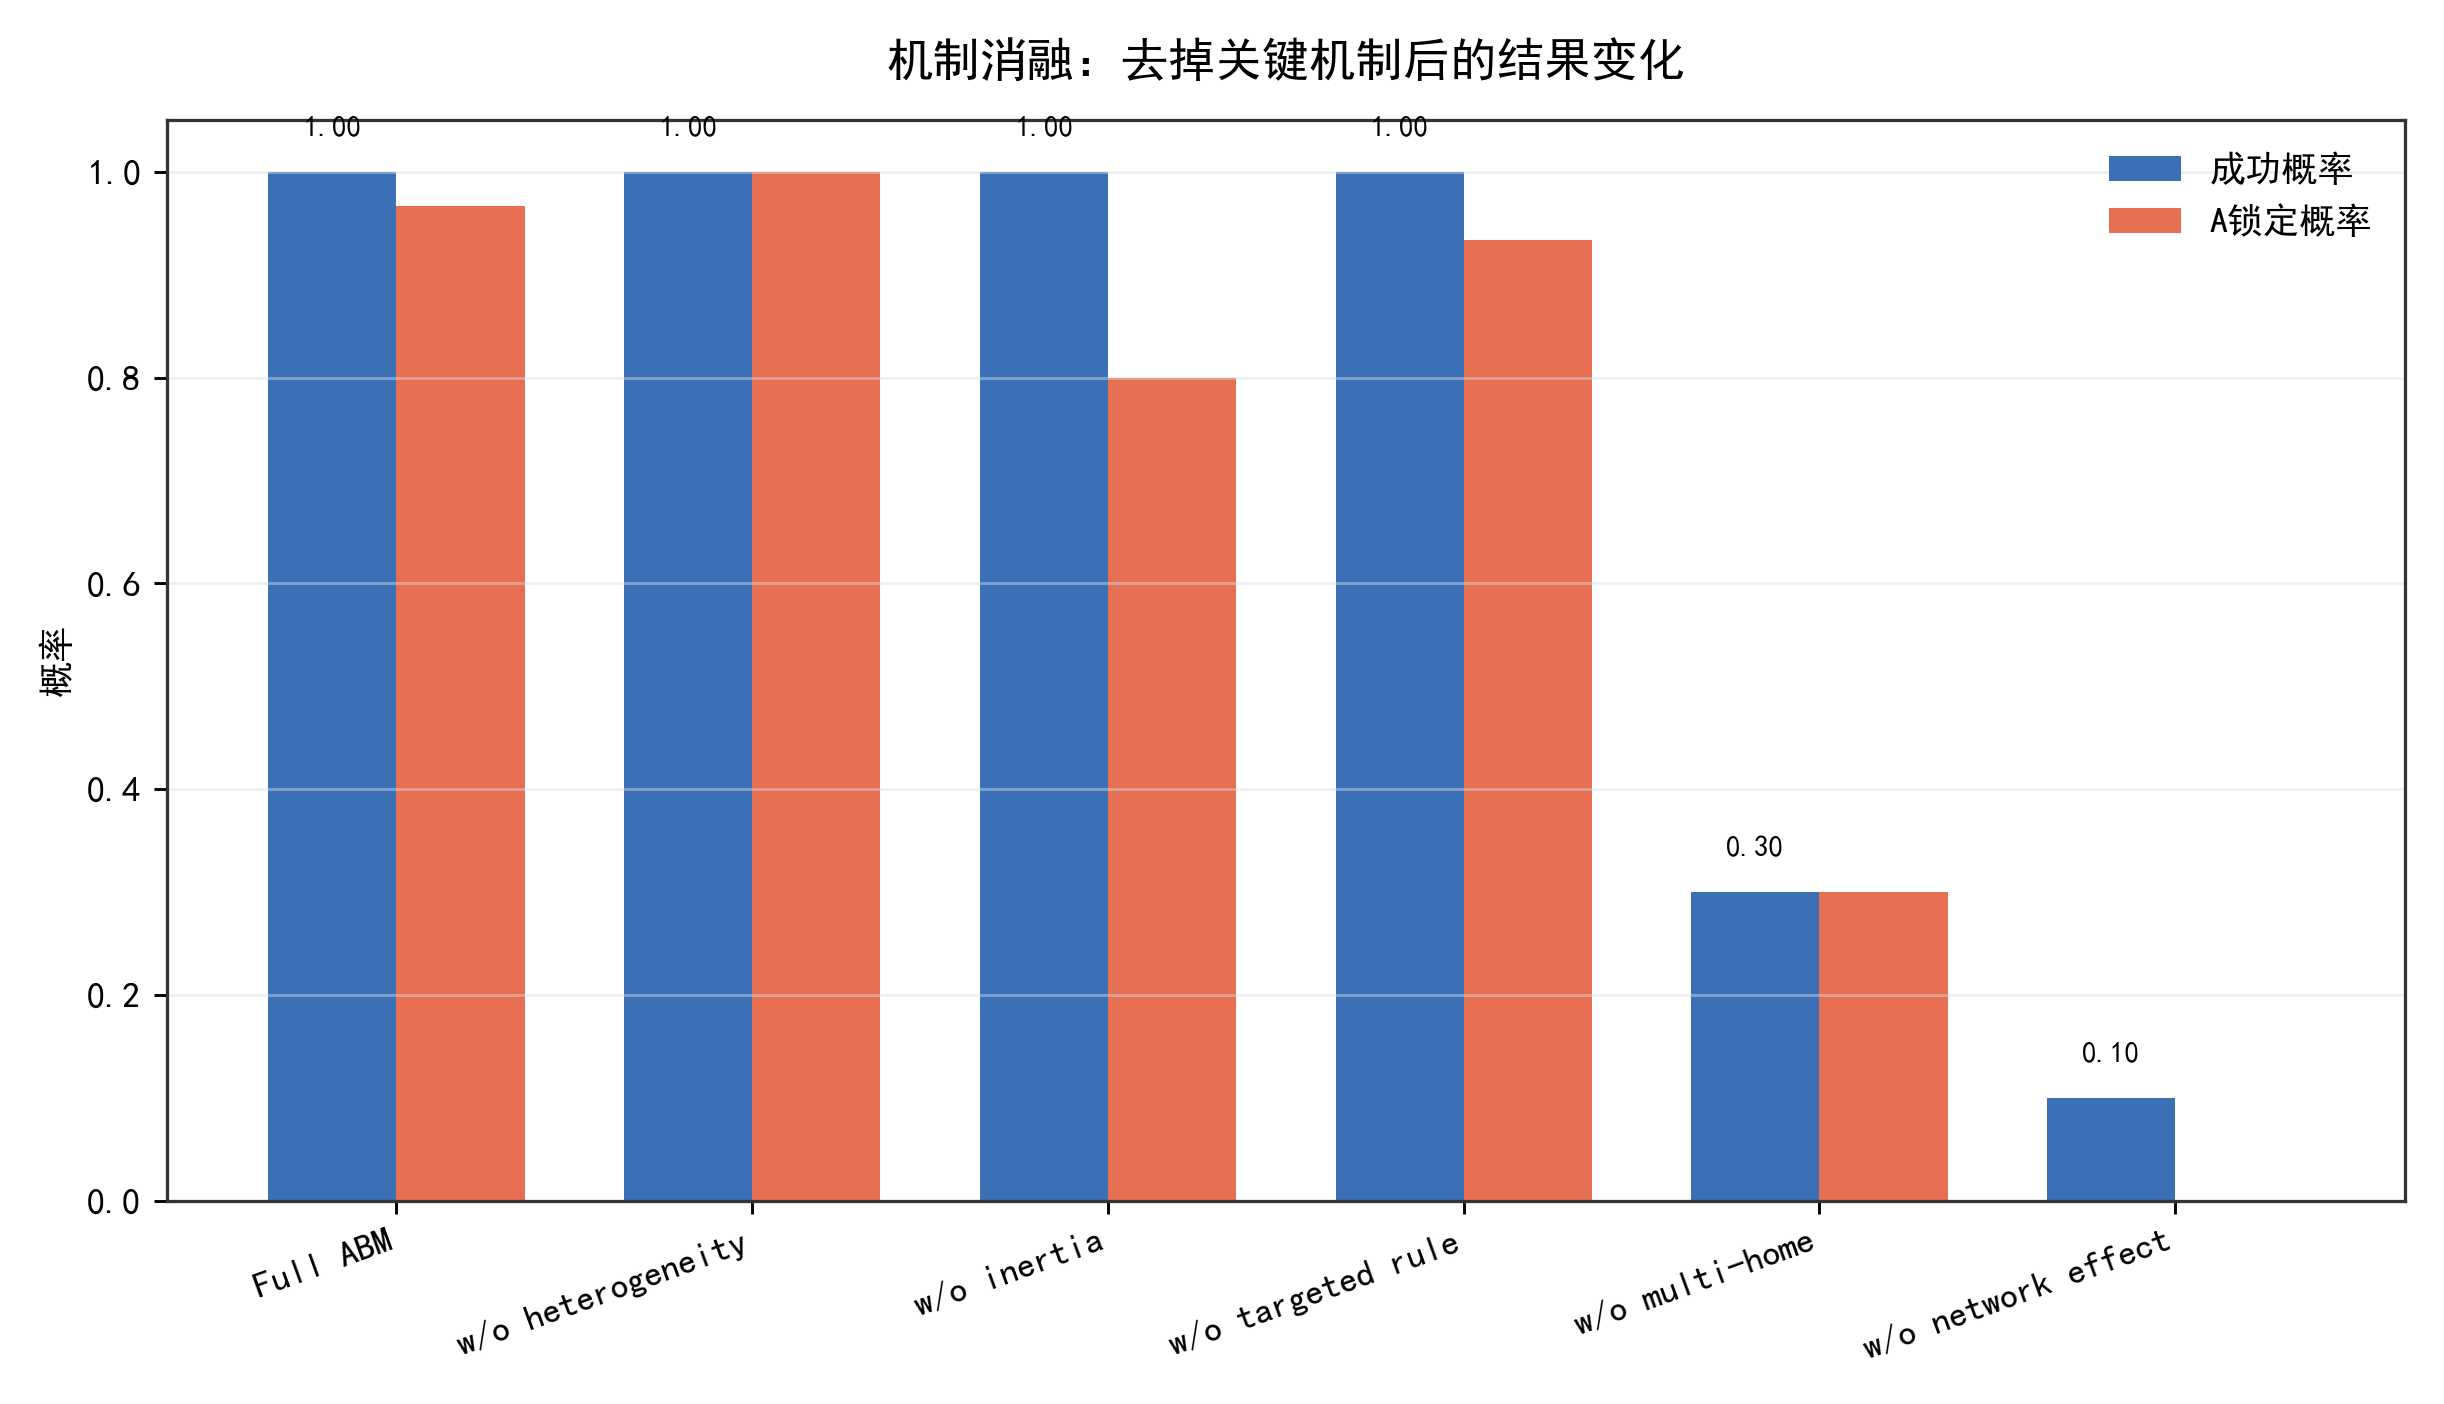
\includegraphics[width=\textwidth]{abm_mechanism_ablation.png}
    \caption{机制消融结果}
  \end{subfigure}
  \hfill
  \begin{subfigure}{0.49\textwidth}
    \centering
    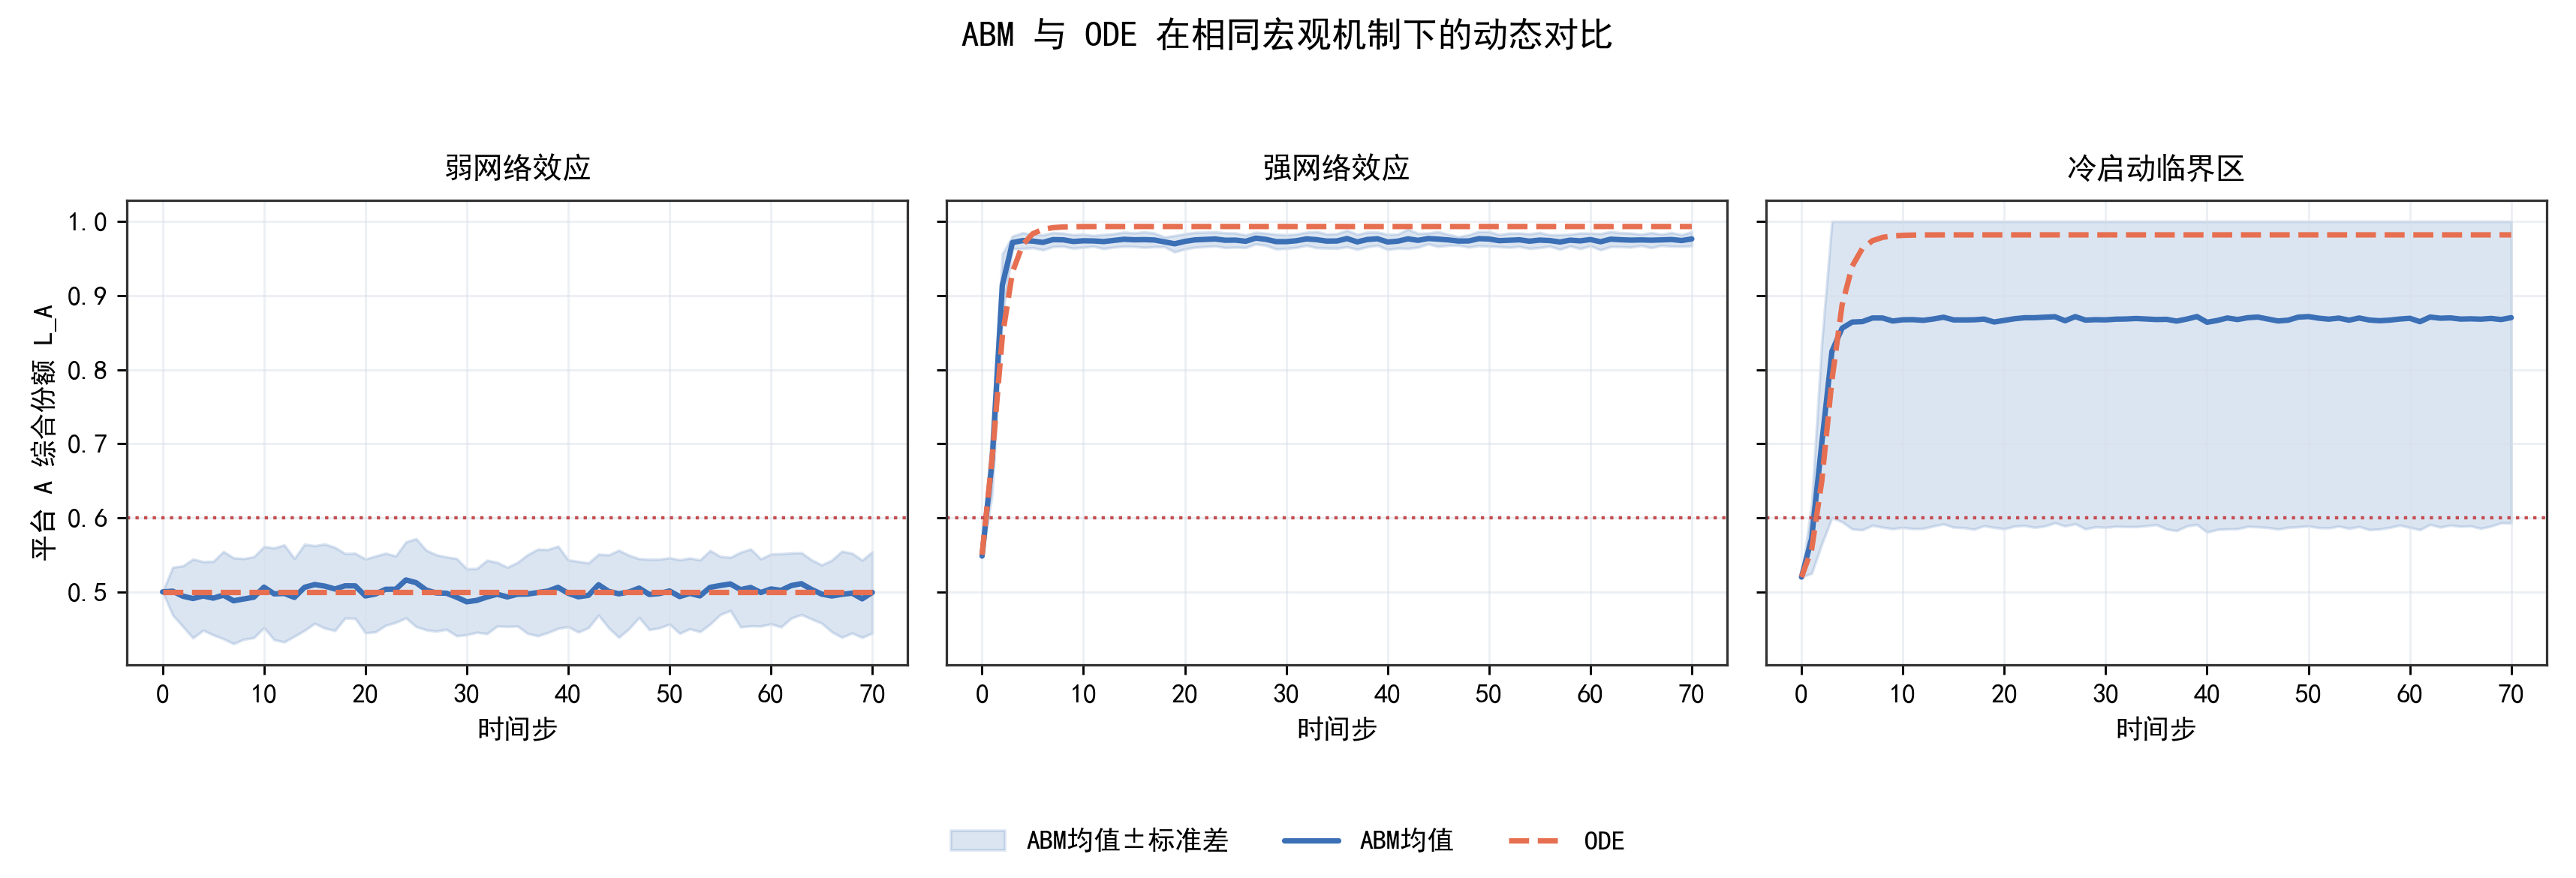
\includegraphics[width=\textwidth]{abm_ode_compare.png}
    \caption{ABM 与 ODE 动态对比}
  \end{subfigure}
  \caption{阶段三补充实验：机制来源与模型关系}
  \label{fig:abm-extra}
\end{figure}

本文还将 ABM 与 ODE 在弱网络效应、强网络效应和冷启动临界区三类场景下进行对比。弱网络效应下，两者均收敛到接近 $L_A=0.5$ 的共存状态；强网络效应下，两者均显示轻微初始优势会被放大为平台 A 锁定。差异主要出现在冷启动临界区：ODE 给出较平滑、确定的跃迁路径，而 ABM 的最终 $L_A$ 标准差达到 0.277，说明同样的宏观参数下仍存在由个体差异和随机路径导致的结果分布。因此，ABM 的价值不在于推翻 ODE，而在于对 ODE 识别出的临界区域进一步估计成功概率、波动范围和机制来源。

\subsection{阶段三结论}

ABM 实验说明，平台竞争结果并非只由平均网络效应决定。个体偏好、补贴敏感度、种子质量、商户多归属能力和随机路径都会改变最终锁定概率。机制消融进一步表明，双边网络效应和商户多归属是弱势平台跨越临界区的主要支撑；ABM 与 ODE 对比则说明，ABM 在保持平均场趋势的同时，能够揭示临界区内的结果分布和路径不确定性。第三阶段将前两阶段的平均场结论扩展到微观机制层面，提高了结论解释力和现实对应性。

\section{综合结论与现实启示}

三个阶段实验共同揭示了双边平台竞争的四个核心规律。

第一，双边正反馈是市场锁定的主要来源。只有用户侧和商户侧网络效应共同存在时，早期优势才会稳定放大。第二，市场演化存在临界阈值。网络效应、服务质量、补贴强度、补贴持续时间和冷启动资源都存在从无效到有效的跃迁区间。第三，补贴策略应服务于跨越临界规模，而不是长期依赖补贴或追求补贴强度最大化。第四，微观主体差异会改变宏观结果，平台必须考虑用户和商户的异质偏好、多平台经营能力与切换成本。

现实平台经营中，新平台或弱势平台应优先获取能够形成双边正反馈的关键用户和关键商户，而非盲目追求单边规模。补贴应更多面向高转化用户和关键供给，避免平均化投放。商户在平台竞争未稳定时应保持适度多归属，以降低被单一平台锁定的风险。用户则应关注平台供给质量、服务稳定性和规则透明度，而不只关注短期补贴。

\section{对题目注意事项的符合性说明}

本项目遵循“从机制出发建立模型”的要求。实验没有依赖真实平台数据拟合，而是基于现实背景、文献机制和合理假设设定参数范围，并通过多组参数扫描、二维热力图、重复随机仿真和敏感性分析解释模型行为。报告关注的是平台共存、倾斜、锁定和逆袭等定性规律，而非精确预测真实市场份额。对于系统行为随参数明显变化的情形，第二阶段和第三阶段均进一步讨论了临界阈值及机制原因。

\begin{thebibliography}{99}

\bibitem{rochet2003}
Rochet, J.-C., \& Tirole, J. (2003). Platform competition in two-sided markets. \textit{Journal of the European Economic Association}, 1(4), 990--1029.

\bibitem{armstrong2006}
Armstrong, M. (2006). Competition in two-sided markets. \textit{The RAND Journal of Economics}, 37(3), 668--691.

\bibitem{parker2005}
Parker, G. G., \& Van Alstyne, M. W. (2005). Two-sided network effects: A theory of information product design. \textit{Management Science}, 51(10), 1494--1504.

\bibitem{katz1985}
Katz, M. L., \& Shapiro, C. (1985). Network externalities, competition, and compatibility. \textit{American Economic Review}, 75(3), 424--440.

\bibitem{arthur1989}
Arthur, W. B. (1989). Competing technologies, increasing returns, and lock-in by historical events. \textit{The Economic Journal}, 99(394), 116--131.

\bibitem{evans2016}
Evans, D. S., \& Schmalensee, R. (2016). \textit{Matchmakers: The New Economics of Multisided Platforms}. Harvard Business Review Press.

\bibitem{wilensky2015}
Wilensky, U., \& Rand, W. (2015). \textit{An Introduction to Agent-Based Modeling: Modeling Natural, Social, and Engineered Complex Systems with NetLogo}. MIT Press.

\bibitem{kazil2020}
Kazil, J., Masad, D., \& Crooks, A. (2020). Utilizing Python for agent-based modeling: The Mesa framework. In \textit{Social, Cultural, and Behavioral Modeling}, Lecture Notes in Computer Science, 12268, 308--317. Springer.

\end{thebibliography}

\end{document}
